


 
\documentclass[11pt]{article}
\usepackage[utf8]{inputenc}
\usepackage{mathtools,amsmath,amssymb}
\usepackage{graphicx}
\usepackage{lmodern}
\usepackage[T1]{fontenc}
%\usepackage{microtype}
\usepackage[pagebackref=false]{hyperref}
\usepackage{bbm}
\usepackage{bm}
\usepackage{appendix}
\numberwithin{equation}{section}



%\usepackage[textsize=tiny]{todonotes}
 
% \usepackage[notref,notcite]{showkeys}
\usepackage{xspace}
%\usepackage{bibentry}
%\usepackage{easybmat}

\usepackage{graphicx}

\usepackage{subcaption} 

%\usepackage[numbers,sort&compress]{natbib}
%\usepackage{hypernat}
 
\usepackage{tikz}
\usetikzlibrary{decorations.pathreplacing}
% MACROS
% % 
% \newcommand{\cristian}[1]{{\bf (* {\color{ForestGreen}V:{} \small #1}*)}}
% \newcommand{\jorge}[1]{{\bf (* {\color{BlueViolet}G:{} \small #1}*)}}
% \newcommand{\rouven}[1]{{ (* {\color{red}{} \small #1}*)}}
 
\frenchspacing

\newcommand{\changelocaltocdepth}[1]{%
  \addtocontents{toc}{\protect\setcounter{tocdepth}{#1}}%
  \setcounter{tocdepth}{#1}%
}
\newcommand{\id}{I}
\newcommand{\Xt}{\tilde{X}}




\newcommand{\len}{L}
\newcommand{\spe}{N}




\setcounter{tocdepth}{2}

\usepackage[margin=2.5cm]{geometry} 

%%%%%  oscillators
\newcommand{\osc}[1]{\mathbf{#1}}
\newcommand{\oscgreek}[1]{\boldsymbol{#1}}
\newcommand{\dagg}[1]{\bar{#1}}
\newcommand{\ep}{\epsilon}
\newcommand{\ob}{\osc{b}}
\newcommand{\oc}{\osc{c}}
\newcommand{\od}{\osc{d}}
\newcommand{\oab}{\dagg{\osc{a}}}
\newcommand{\obb}{\dagg{\osc{b}}}
\newcommand{\ocb}{\dagg{\osc{c}}}
\newcommand{\odb}{\dagg{\osc{d}}}
\newcommand{\ox}{\oscgreek{\xi}}
\newcommand{\oxb}{\dagg{\oscgreek{\xi}}}
\newcommand{\och}{\oscgreek{\chi}}
\newcommand{\ochb}{\dagg{\oscgreek{\chi}}}
\newcommand{\NN}{\mathbf{N}}
\newcommand{\ccc}{\mathbf{C}}
\newcommand{\qop}{Q}
\newcommand{\sop}{Y}
\newcommand{\q}{\mathbf{\epsilon}}
\newcommand{\ID}{I}
\newcommand{\per}{P}

\newcommand{\EE}{\mathrm{E}}

\newmuskip\pFqmuskip

\newcommand*\pFq[6][8]{%
  \begingroup % only local assignments
  \pFqmuskip=#1mu\relax
  \mathchardef\normalcomma=\mathcode`,
  % make the comma math active
  \mathcode`\,=\string"8000
  % and define it to be \pFqcomma
  \begingroup\lccode`\~=`\,
  \lowercase{\endgroup\let~}\pFqcomma
  % typeset the formula
  {}_{#2}\phi_{#3}{\left[\genfrac..{0pt}{}{#4}{#5};#6\right]}%
  \endgroup
}
\newcommand{\pFqcomma}{{\normalcomma}\mskip\pFqmuskip}


\DeclareMathOperator{\tr}{tr}
\DeclareMathOperator{\Li}{Li}
\DeclareMathOperator{\diag}{diag}


\newcommand{\KL}{\mathcal{K}}
\newcommand{\KR}{\hat{\mathcal{K}}}
\newcommand{\oa}{\mathbf{a}}

\newcommand{\oad}{\mathbf{a}^{\dagger}}

\newcommand{\phil}{\beta_-}
\newcommand{\phir}{\beta_+}
\newcommand{\ma}{n}

\newcommand{\oaq}{\mathbf{a}_\q}

\newcommand{\oadq}{\mathbf{\bar{a}}_\q}

\newcommand{\N}{\mathbf{N}}
\newcommand{\twoj}{\nu}



\begin{document} 
 
\begingroup
% \centering
\begin{center}
 \begingroup\LARGE
\bf Stirring process
\par\endgroup
 \vspace{3.5em}
 \begingroup\large \bf
% {Rouven Frassek}
 \par\endgroup
\vspace{2em}

\begingroup\sffamily 
%  
% Università degli Studi di Modena e Reggio Emilia
%University of Modena and Reggio Emilia, 
%\\Department of Physics, Informatics and Mathematics,\\
%Via G. Campi 213/b, 41125 Modena, Italy\\ 
\par\endgroup
\vspace{2em}

 Version: \today
\end{center}
%  

\thispagestyle{empty}

\begin{abstract}
\noindent
...
\end{abstract}

%\vfill 

\tableofcontents

% \newpage

\section{Introduction} 
In the past years duality has been developed to study stochastic processes, especially in the boundary driven case, i.e. when the system is put in contact with boundaries that generate a non-equilibrium current. The literature is huge. We can address , for instance, to \cite{giardina2009duality,carinci2013duality,frassek2020duality}. One application of duality is the attempt to characterize the non equilibrium steady state of boundary driven process via the so called absorption probabilities. Indeed, there are many cases where the dual process has absorbing boundaries. This means that the the chain is eventually empty in the long time scale. Moreover, there are cases in which the steady state of a stochastic process can be computed explicitly, thanks to the integrability property of the system (quantum inverse scattering method, matrix product ansatz). In this direction, some examples can be found in \cite{derrida1993exact,frassek2019non,frassek2020eigenstates}. In the past, the focus has been on processes where one can distinguish, in each site of a certain graph, a (or many) particles or an empty state. However, this particles are indistinguishable, in the sense that you can pile up in a site just one type of particles. Some natural questions arise: what happens if we imagine to assign different colours to the particles? Is the duality property still holding? How far can we push our analysis for the characterization of the non equilibrium steady state?\\
The way one can define a multi-type (or multi-species) interacting particle system is not unique. In the literature there are many. Two of them are the following. On one hand, the \textit{multi-layer models}, in which the process is constructed on a many layer graph where each graph correspond to a type and perform a kind of dynamic (independent jump, exclusion/inclusion walkers) and the layers communicate each other with some "switching probabilities". The state space of the Markov process is the Cartesian product of the state spaces of each layer, i.e. of the two species. For example see \cite{floreani2022switching,redig2022ergodic}. On the other hand, the \textit{single layer models}. Here, there is just one layer, where particles of each type can pile up, in a way that the exclusion dynamic concerns many species together. In other words, now the species can interact "directly", not just by switching layer. Here the state space contains all the species and it is not product anymore. Some examples of such a dynamic can be found in \cite{casini2022uphill,vanicat2017exact,zhou2021orthogonal}. \\
In this work we concentrate our effort in this last "single layer" case with a repulsive process, i.e. a dynamic in which a maximum amount of particles can be present in each site at each time. We will call this amount, the "maximal occupancy" and it will indicated with $\twoj$ where $\twoj\in\mathbb{N}$. Particle of any species can exchange their position in the graph, under this exclusion constraint. The system will be put out of equilibrium and some absorbing duality result are investigated. Moreover, we will use this duality, to study the out of equilibrium steady state. In particular, in case of $\twoj=1$ we should retrieve the model studied in \cite{vanicat2017exact}. We will then exploit this last result and the duality, to write explicitly all the correlations of this \textit{hard-core exclusion} case. The main tool that we will use is the Lie algebraic description of the process, that allows to find the duality as a proper symmetry of the generator. 
\paragraph{Organization of the paper}
\section{The stirring process}
We consider the stirring process with an arbitrary number of particles $N$. It is important to note that any one of them can be considered the empty (or hole) particle. Thus, in this first general setting we do not distinguish between real and empty particles. However, this distinction will be useful in the section about duality, where we will see that this empty will play a special role. The stochastic dynamics is Markovian and consist in an exchange of particles of any type between two connected site of a graph. \\
\subsection{The infinitesimal generator}
Let's consider a connected and undirected graph $G=(V,\mathcal{E})$ where $x\in V$ denotes the set of vertex and $\mathcal{E}$ denotes the set of edges $(x,y)$ with $x,y\in V$.  The process has a repulsive nature, thus the state space must contain informations about this maximal occupancy. Then we define 
\begin{equation}\label{stateSpace}
    \Omega:=\left\{n=(n_{1},\ldots,n_{N})\in\mathbb{N}_0^{N}\;:\; |n|=\twoj\right\}^{|V|}
\end{equation}
where $|n|=\sum_{k=1}^{N}n_{k}$ denotes the total number of particles per site and $|V|$  the total number of vertices. At each site $x\in V$, we describe the occupation with an $N-$dimensional vector in which the value of the $k$-th component $n_{k}^{x}$ denotes the number of particles of species $k$, under the constraint that the total number of particle in the site is $\twoj$. \\
The dynamic consists in an exchange of particles between connected vertex. Moreover, each vertex can be connected with a reservoir that inject, remove or exchange particles. Mathematically, this can be described by an infinitesimal generator as follows
\begin{equation}\label{Generator}
    \mathcal{L}=\sum_{(x,y)\in \mathcal{E}}\omega_{x,y}\mathcal{L}_{x,y}+\sum_{x\in V}\Gamma_{x}\mathcal{L}_{x}
\end{equation}
where the quantities $ \omega_{x,y}$ are called conductancies and $\Gamma_{x}$ local inhomogeneities. The generator $\mathcal{L}_{x,y}$ is called the \textit{edge generator}, while $\mathcal{L}_{x}$ is called the \textit{site generator}. These linear operators act on local functions $f:\Omega\to \mathbb{R}$ as follows
\begin{equation}
\mathcal{L}_{x,y}f(n)=\sum_{k,l=1}^{N}n_{k}^{x}n_{l}^{y}\left[f(n-\delta_{x}^{k}+\delta_{l}^{x}+\delta_{k}^{y}-\delta_{l}^{y})-f(n)\right]
\end{equation}
\begin{equation}
    \mathcal{L}_{x}f(n)=\sum_{k,l=1}^{N}\alpha_{k}^{x}n_{l}^{x}\left[f(n+\delta_{k}^{x}-\delta_{l}^{x})-f(n)\right]
\end{equation}
where 
$\delta_{k}^{x}=(0,\ldots,0,1,0,\ldots,0)$ withe the one in the $k$-th position. This means that the edge generator exchanges a particle of type $k$ in the site $x$ with a particle of type $l$ in the site $y$, while the site generator inject a particle of type $k$ and remove a particle of type $l$, both in the site $x$. The following Figure \ref{fig:1}, Figure \ref{fig:2} help in understanding the dynamics. 
\begin{figure}
    \centering
    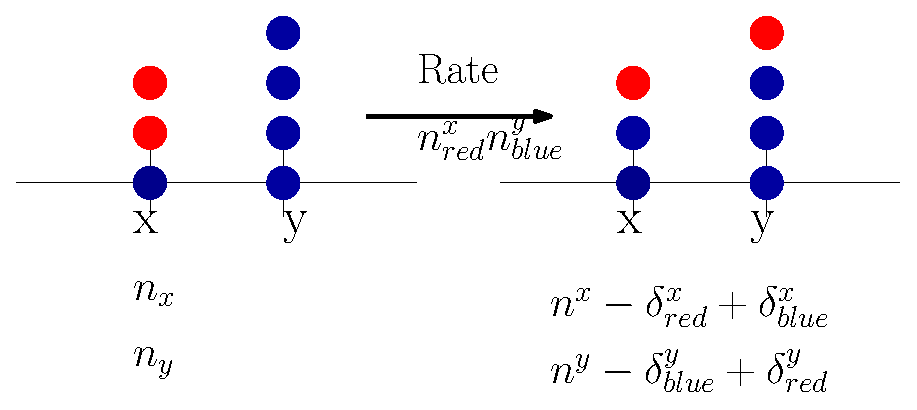
\includegraphics[scale=0.6]{Dyn_stir.eps}
    \caption{The edge dynamics}
    \label{fig:1}
\end{figure}
\begin{figure}
    \centering
    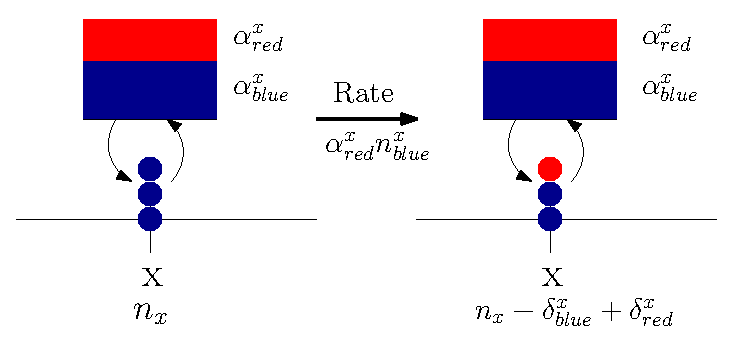
\includegraphics[scale=0.88]{Dyn_stir_bordo.eps}
    \caption{The site dynamics}
    \label{fig:2}
\end{figure}\newline \\
\textbf{Remark}: 
    We can always assign the name "empty" to one of the species of particles in the above dynamics (let's say, without loss of generality, the species 1). This species would play the role of "compensator" in the exclusion constraint, in the sense that its occupation will always be determined once we know the others, i.e. $\forall x\in V$: 
    \begin{equation}
        n_{1}^{x}=\twoj-\sum_{k=2}^{N}n_{k}^{x}
    \end{equation}
    Moreover, if we set $N=2$ and $\twoj=2j$, we exactly retrieve the SEP(2j), where the empty occupation is indeed $2j-\eta_{x}$ where $\eta_{x}$ is the number of (color blind) particles in the site $x$. In this sense we can think about the stirring process as the natural generalization of the SEP(2j).
    \begin{flushright}
        $\square$
    \end{flushright}
The process described by \eqref{Generator} is reversible if and only if, for any $k\in\{1,\ldots,N\}$, the boundary parameters $\alpha_{k}^{x}=\alpha_{k}$ $\forall x\in V$. The reversible product measure is a Multinuomial distribution of parameter $\twoj$. That means that 
\begin{equation}\label{reversibleMeasure}
    \mu^{rev}=\bigotimes_{x\in V}\mu^{rev}_{x}\qquad \mu_{x}^{rev}\sim \text{Multinomial}\left(\twoj,p_{1},\ldots,p_{N}\right)\quad :\quad p_{k}=\frac{\alpha_{k}}{\sum_{i=1}^{N}\alpha_{i}}
\end{equation}
This can be proven just by imposing the detailed balance conditions for the edge and for the site generators. Let us notice that the reversible measure is product only over the sites, but not over the species. This is due to the exclusion constraint that makes particle interact. 

{\color{red}[LET'S SKIP THE PROOF? I THINK IT IS STANDARD!]}.\\
\subsection{The Lie algebraic description}



%The approach we use to find duality relations is the Lie algebraic one. The main idea is to describe the infinitesimal generator (or better, its transposed, i.e. the Hamiltonian operator) via a proper combination of the basis of a certain Lie algebra. Then, duality will be found by symmetry argument.\\


Consider the $gl(N)$ Lie algebra with with generators denoted by $\EE_{a,b}$ with $a,b\in \{1,\ldots,N\}$ and commutation relations
\begin{equation}\label{eq:comgl}
\left[\EE_{ab},\EE_{cd}\right]=\EE_{ad}\delta_{bc}-\EE_{cb}\delta_{ad}\qquad \forall a,b\in \{1,\ldots,N\}
\end{equation}
The finite-dimensional representations are labelled by partitions $\lambda=(\lambda_1,\lambda_2,\ldots,\lambda_N)$ with $\lambda_i\in \mathbb{N}$ and  $\lambda_i\geq \lambda_{i+1}$.
We are interested in the symmetric finite-dimensional representations with 
\begin{equation}\label{eq:dynkin}
    \lambda=(\twoj,0,\ldots,0) \qquad\text{where}\qquad \twoj\in\mathbb{N}
\end{equation} 
The dimension of the symmetric representations is given by the combination of $N$ objects in $\twoj$ positions with repetition:
\begin{equation}
	D= \frac{(N+\twoj-1)!}{\twoj  !(N-1)!}
\end{equation} 
The basis elements of the vector space of the representation $\mathbb{C}^{D}$ are denoted by 
\begin{equation}
  |n\rangle=  |n_{1},\ldots,n_{N}\rangle\qquad \forall
    n=(n_{1},\ldots,n_{N})
\end{equation}
$\forall n=(n_{1},\ldots,n_{N})\in \chi$ where $\chi:=\left\{n:|n|=\twoj\right\}$ {\color{red}(let us notice that $\Omega=\chi^{|V|}$)?}. This vector can be mapped in a one-to-one correspondence with the canonical basis of $\mathbb{C}^{D}$. This basis vector satisfy the orthogonality relation
\begin{equation}\label{ortho}
    \langle m_{1},\ldots,m_{N}|n_{1},\ldots,n_{N}\rangle=\prod_{k=1}^{N}\delta_{m_{k},n_{k}}
\end{equation}
where  $ \langle m_{1},\ldots,m_{N}|=| m_{1},\ldots,m_{N}\rangle^T$.
 
The explicit actions of the basis element of the algebra on the vectors of the space $\mathbb{C}^{D}$ are the following, for non Cartan and Cartan elements respectively: 
\begin{equation}\label{actionE}
	\begin{cases}
		E_{ab}|n_{1},\ldots,n_{a},\ldots,n_{b},\ldots,n_{N}\rangle =n_{b}|n_{1},\ldots,n_{a}+1,\ldots,n_{b}-1,\ldots,n_{N}\rangle\\[0.1cm]
		E_{aa}|n_{1},\ldots,n_{a},\ldots,n_{b},\ldots,n_{N}\rangle = n_{a} |n_{1},\ldots,n_{a},\ldots,n_{b},\ldots,n_{N}\rangle
	\end{cases}\qquad \forall a,b\in\{1,\ldots,N\}
\end{equation}  
One can check that the generators defined in this way satisfy the commutation relations \eqref{eq:comgl} and yield Dynkin weight \eqref{eq:dynkin}.


We now define the equivalent of \eqref{stateSpace} in the vector notation
 \begin{equation}
	\Omega':=\left\{|n\rangle=|n_{1},\ldots,n_{N}\rangle \;:\;n\in\mathbb{N}_0^N,\;\;|n|=\twoj\right\}^{\otimes|V|}
	\end{equation}
where we denote 
\begin{equation}
|{\bf n}\rangle=\left(\,\bigotimes_{x\in V}	|n_{1},\ldots,n_{N}\rangle_{x}\right)\in \Omega'
\end{equation}
such that
\begin{equation}
    \langle {\bf n}|{\bf m}\rangle =\prod_{x=1}^L\prod_{i=1}^N\delta_{n^x_i,m^{x}_i}
\end{equation}


When the state space is discrete, it is useful to write the dynamics of the process in term of an other operator, the Hamiltonian. The relation between these two operator is the following
\begin{equation}
H=\mathcal{L}^{T}
\end{equation}




Following  \cite{belitsky2015self} we define
\begin{equation}
    \mathcal{L}f( {\bf n})=\langle f|H| {\bf n}\rangle
\end{equation}
where 
\begin{equation}
    \langle f|=\sum_{ {\bf n}}f( {\bf n})\langle  {\bf n}|
\end{equation}


The Hamiltonian operator can be written in term of the basis element of the Lie algebra as

\begin{equation}\label{OriginalHamiltonian}
	\begin{split}
		H=\sum_{x,y\in \mathcal{E}}\omega_{x,y}H_{x,y}+\sum_{x\in V}\Gamma_{x}H_{x}
	\end{split}
\end{equation}
where the edge Hamiltonian is
\begin{equation}\label{edgeHamiltonian}
H_{x,y}=\sum_{k,l=1}^{N}\left(E_{kl}\otimes E_{lk}-E_{ll}\otimes E_{kk}\right)_{x,y}
 \end{equation}
 and where the site Hamiltonian is
 \begin{equation}\label{siteHamiltonian}
H_{x}=\sum_{k,l=1}^{N}\alpha_{k}^{x}\left(E_{kl}-E_{ll}\right)_x
\end{equation}


Moreover, by the \eqref{coproductC2} and by computing the explicit action of the diagonal part, we can write this Hamiltonian in function of the coproduct of the second Casimir
\begin{equation}
    C_{2}=\sum_{a,b=1}^{N}E_{ab}E_{ba}
\end{equation}
It reads
\begin{equation}
	H=\sum_{x,y\in \mathcal{E}}\omega_{x,y}\left\{\frac{1}{2}\Delta(C_{2})-\twoj(2\twoj+N)\frac{1}{2}\mathbbm{1}\otimes\mathbbm{1}\right\}+\sum_{x\in V}\Gamma_{x}\sum_{k,l=1}^{N}\alpha_{k}^{x}\left(E_{k,l}-\twoj\mathbbm{1}\right)
\end{equation}
Here we introduced the standard coproduct $\Delta:E_{ab}\mapsto E_{ab}\otimes \mathbbm{1}+\mathbbm{1}\otimes E_{ab}$ and used that $C_{2}=\twoj(\twoj+N)$. 

 
\textbf{Remark}: The symmetric representations $\lambda=(\twoj,0,\ldots,0)$ are dual to the representations $\lambda=(\twoj,\ldots,\twoj,0)$ that can be obtained via 
\begin{equation}
   \bar E_{ab}=\mu\delta_{ab}-E_{N-b+1,N-a+1}
\end{equation}
{\color{red} This needs to be checked and give alternative form of Hamiltonian?}


\section{Duality}
Consider two Markov processes $(\eta_{t})_{t\geq 0}$ on a state space $\Omega$ and $(\xi_{t})_{t\geq 0}$ on a state space $\widetilde{\Omega}$. We say that they are dual, with respect to a duality function $D:\Omega\times \widetilde{\Omega}\to \mathbb{R}$ if $\forall \eta\in \Omega$, $\forall \xi\in \widetilde{\Omega}$ and $\forall t\geq 0$ we have 
\begin{equation}
    \mathbb{E}_{\eta}\left[D(\eta_{t},\xi)\right]=\mathbb{E}_{\xi}\left[D(\eta,\xi_{t}\right]
\end{equation}
Moreover, if $\eta_{t}$ and $\xi_{t}$ are the same process, we talk about \textit{self-duality} and \textit{self-duality function}. The duality property can also be characterized by a relation with the generators. Let $\mathcal{L}$ be the generator of $\eta_{t}$ and let $\mathcal{L}_{dual}$ be the generator of $\xi_{t}$, then we say that two process are in a duality relation if 
\begin{equation}
    \left(\mathcal{L}D(\cdot,\xi)\right)(\eta)=\left(\mathcal{L}_{dual}D(\eta,\cdot)\right)(\xi)
\end{equation}
\subsection{Algebraic formulation}
In particular, if the process has a countable space, the duality is a matrix, and we can rewrite the above relation with the Hamiltonians has follows
\begin{equation}\label{dualityHamiltonian}
    H^{T}D=DH_{dual}
\end{equation}
By \eqref{dualityHamiltonian}, we can see the duality matrix as a similarity transformation between the original and the dual Hamiltonian. \\
We now construct our main result: \textit{the process defined in \eqref{Generator} is self dual with absorbing boundaries}. Thus, we have to construct a duality matrix $D$ and an Hamiltonian $H_{dual}$ in order to fulfill the equation \eqref{dualityHamiltonian}.
\\
The self-dual process is defined in the self-dual state space 
\begin{equation}\widetilde{\Omega}:=\Omega\times \mathbb{N}_{0}^{|V|}\end{equation} with elements
\begin{equation}
	|\xi\rangle=\bigotimes_{x\in V}\left(|r_{0},\ldots,r_{N}\rangle_{x}\otimes |m_{1}^{\varepsilon(x)},\ldots,m_{N}^{\varepsilon(x)}\rangle_{x}\right)
\end{equation}
The self-dual Hamiltonian is the following
\begin{equation}
	\begin{split}
		H=\sum_{x,y\in \mathcal{E}}\omega_{x,y}H_{x,y}+\sum_{x\in V}\Gamma_{x}\widetilde{H}_{x,\varepsilon(x)}
	\end{split}
\end{equation}
where
\begin{align}
H_{x,y}&=\sum_{k,l=1}^{N}\left(E_{kl}^{x}\otimes E_{lk}^{y}-E_{ll}^{x}\otimes E_{kk}^{y}\right)\\
\widetilde{H}_{x,\varepsilon(x)}&=\left(\sum_{i=2}^{N}\alpha_{i}^{x}\right)\sum_{k=2}^{N}\left((a^{\dagger}_{k})_{\varepsilon(x)}E_{1k}^{x}-E_{kk}^{x}\right)
\end{align}
and where  $(a^{\dagger}_{k})_{\varepsilon(x)}$ is a bosonic creation operator acting on an extra site attached to $x$ and denoted by $\varepsilon(x)$. Let us notice that edge part of the dual Hamiltonian is exactly the one of \eqref{edgeHamiltonian} (self-duality). The site part only replace any particle of type $k\in \{2,\ldots,N\}$ with a type $1$  and put them into an extra site, attached to $x$. Dual particles of type $k$ are piled up into an this extra site, and they leave the graph forever. This means that the species $1$ plays a special role in the duality. If we think about this $1$ species as the empty, we can interpret the dual process as an absorbing dual, i.e. a process that eventually empties the graph.\\
Associated with this dual process there is the following duality matrix 
\begin{equation}\label{dualityMatrix}
	D=\prod_{x\in V}\left(\sum_{m_{2}^{\varepsilon(x)},\ldots,m_{N}^{\varepsilon(x)}=0}^{\infty}\prod_{k=2}^{N}\left(\frac{\alpha_{k}^{x}}{\alpha_{0}^{x}+\ldots+\alpha_{N}^{x}}\right)^{m_{k}^{\varepsilon(x)}}\langle m_{2},\ldots,m_{N}|_{\varepsilon(x)}\otimes R_{x}e^{E}_{x} \right)
	=\prod_{x\in V}\left(D_{\varepsilon(x)}\otimes D_{x}\right)
\end{equation}
where we define the \textit{symmetry operator} as
\begin{equation}\label{e_def}
	E=\sum_{a=2}^{N}e_{a1}
\end{equation}
and the \textit{cheap duality matrix} as 
\begin{equation}
	R^{-1}_{x}=\sum_{n\in \chi}\frac{(2j)!}{n_{1}^{x}!\ldots n_{N}^{x}!}|n_{1},\ldots,n_{N}\rangle_{x}\langle n_{1},\ldots,n_{N}|_{x}%\quad \forall n\in \chi
\end{equation}
Moreover, the element of the matrix \eqref{dualityMatrix} are given by
\begin{equation}\label{dualityElements}
	D(n,\xi)=\langle n|D|\xi\rangle=\prod_{x\in V}\left(\frac{(2j-\sum_{k=2}^{N}r_{k}^{x})!}{(2j)!}\prod_{k=2}^{N}\frac{n_{k}^{x}!}{(n_{k}^{x}-r_{k}^{x})!}\left(\frac{\alpha_{k}}{\alpha_{1}+\ldots+\alpha_{N}}\right)^{m_{k}^{\varepsilon(x)}}\right)
\end{equation}
\subsubsection{Proof of the duality relation}
\textbf{The transposition property of the cheap duality}: \\
This cheap duality matrix has the following \textit{transposition property}:
\begin{equation}\label{transpositionR}
	\left(e_{ba}\right)^{T}=R e_{ab}R^{-1}\quad \forall a,b\in\{0,1,\ldots,N\}
\end{equation}
Indeed, for any configuration $\mathbf{n},\mathbf{r}\in \Omega$, by using \eqref{matrixFormulaE} we obtain
\begin{align*}
	R e_{ab}R^{-1}=&\sum_{r\in\chi}\left(\frac{r_{1}!\ldots r_{N}!}{(2j)!}|r_{1},\ldots,r_{N}\rangle \langle r_{1},\ldots, r_{N}|\right)
	\\&
	\sum_{s\in \chi,}\left(s_{b}|s_{1},\ldots,s_{a}+1,\ldots,s_{b}-1,\ldots s_{N}\rangle \langle s_{1},\ldots,s_{N}|\right)
	\\&
	\sum_{n\in\chi}\left(\frac{(2j)!}{n_{1}!\ldots n_{N}!}|n_{1},\ldots,n_{N}\rangle \langle n_{1},\ldots, n_{N}|\right)=
	\\&
	\sum_{r,n\in \chi}\frac{r_{1}!\ldots r_{N}!}{(2j)!}|r_{1},\ldots,r_{N}\rangle \langle r_{0},\ldots, r_{N}|
	\frac{(2j)!}{n_{1}!\ldots n_{N}!}n_{b}|n_{1},\ldots,n_{a}+1,\ldots,n_{b}-1,\ldots n_{N}\rangle \langle n_{1},\ldots,n_{N}|=\diamond
\end{align*}
By using orthogonality relation \eqref{ortho}\begin{align*}
\diamond=&\sum_{r\in \chi}\frac{r_{1}!\ldots r_{N}!}{(2j)!}\frac{(2j)!}{r_{1}!\ldots (r_{a}-1)!\ldots(r_{b}+1)!\ldots r_{N}!}(r_{b}+1)|r_{1},\ldots,r_{N}\rangle \langle r_{0},\ldots,r_{a}-1,\ldots,r_{b}-1,\ldots,r_{N}|
	\\=&\sum_{r\in\chi}\frac{r_{1}!\ldots r_{N}!}{(2j)!}\frac{(2j)!}{r_{1}!\ldots (r_{a}-1)!\ldots(r_{b}+1)!\ldots r_{N}!}(r_{b}+1)\frac{r_{a}}{r_{a}}|r_{1},\ldots,r_{N}\rangle \langle r_{1},\ldots,r_{a}-1,\ldots,r_{b}-1,\ldots,r_{N}|
	\\=&\sum_{r\in \chi}
	r_{a}|r_{1},\ldots,r_{N}\rangle \langle r_{1},\ldots,r_{a}-1,\ldots,r_{b}-1,\ldots,r_{N}|
	\\=&
	\left(e_{ba}\right)^{T}
\end{align*}
\textbf{The edge self-duality}\\
The second Casimir $C_{2}$ is a central element of $gl(N)$. Thus, every element of $gl(N)$ is a symmetry of $C_{2}$.
Let's chose the operator $E$ defined in \eqref{e_def}, then $\Delta(E)$ is a symmetry of $\Delta(C_{2})$.
In order to preserve a product structure of the duality matrix, we make the symmetry exponential:
\begin{equation}\label{Simmetry_s}
	S=e^{\Delta(E)}
\end{equation}
By considering two sites $x,y$:
\begin{equation}
	\begin{split}
		S&=e^{\Delta(E)}=e^{(\mathbbm{1}\otimes E+E\otimes \mathbbm{1})}=e^{\mathbbm{1}\otimes E}e^{E\otimes \mathbbm{1}}=\sum_{k=0}^{N}\frac{\left(\mathbbm{1}\otimes E\right)^{k}}{k!}\sum_{j=0}^{N}\frac{\left(E\otimes \mathbbm{1}\right)^{j}}{j!}
		\\&=
		\left(\mathbbm{1}\otimes \sum_{k=0}^{N}\frac{E^{k}}{k!}\right)\left(\sum_{j=0}^{N}\frac{E^{j}}{j!}\otimes \mathbbm{1}\right)=\left(\mathbbm{1}\otimes e^{E}\right)\left(e^{E}\otimes \mathbbm{1}\right)=e^{E}\otimes e^{E}
		\\&=e_{x}^{E} e^{E}_{y}
	\end{split}
\end{equation}
Since the Hamiltonian \eqref{OriginalHamiltonian}, can be written as a linear function of the coproduct of the second Casimir, we have \begin{equation}[H_{x,y},e^{\Delta (C_{2})}]=0\end{equation} and thus \begin{equation}\label{symmetryH-C}[H_{x,y},e^{E}_{x}e^{E}_{y}]=0\end{equation} then the operator \eqref{Simmetry_s} is also a symmetry for the Hamiltonian. 
Since the duality matrix \eqref{dualityMatrix} is product over the vertex of the graph it is enough to prove that $\forall x,y\in \mathcal{E}$:
\begin{align}
	H_{x,y}^{T}D=DH_{x,y}\label{bulkDuality}
\end{align}
For a fixed edge we only have $D_{x}D_{y}$. 
\begin{align*}
	H_{x,y}^{T}D&=D_{\varepsilon(x)}D_{\varepsilon(y)}\otimes R_{x}R_{y}H_{x,y}R_{x}^{-1}R_{y}^{-1}R_{x}R_{y}e^{E}_{x}e^{E}_{y}\prod_{z\neq x,y}D_{e(z)}D_{z}
	\\&=
	D_{\varepsilon(x)}D_{\varepsilon(y)}\otimes R_{x}R_{y}H_{x,y}e^{E}_{x}e^{E}_{y}\prod_{z\neq x,y}D_{e(z)}D_{z}
\end{align*} 
By exploiting \eqref{symmetryH-C}
\begin{align*}
	H_{x,y}^{T}D&=	D_{\varepsilon(x)}D_{\varepsilon(y)}\otimes R_{x}R_{y}e^{E}_{x}e^{E}_{y}\prod_{z\neq x,y}D_{e(z)}\otimes D_{z}H_{x,y}=
	DH_{x,y}
\end{align*}
thus (\ref{bulkDuality}) is proved.\\
\textbf{The site absorbing duality}\\
For the sake of notation we remove the superscripts "$x$" from the operators $E_{ab}$ and from the reservoirs densities $\alpha_{k}$. Exploiting again the product form of the duality matrix we can just show that, $\forall x\in V$ the following relation is true 
\begin{equation}\label{boundaryDuality}
    	H_{x}^{T}D=D\widetilde{H}_{x,\varepsilon(x)}
\end{equation}
For the sake of notation and without loss of generality we restrict to the case where $N=3$. \\
The transpose of the single site Hamiltonian reads as
\begin{equation}
	\begin{split}
	H_{x}^{T}&=\sum_{k=1}^{3}\alpha_{k}\left[E_{kl}-E_{ll}\right]^{T}\\&=
	\alpha_{1}\left[E_{12}-E_{22}\right]^{T}+\alpha_{1}\left[E_{13}-E_{33}\right]^{T}+\alpha_{2}\left[E_{21}-E_{11}\right]^{T}\\&+\alpha_{2}\left[E_{23}-E_{33}\right]^{T}+
	\alpha_{3}\left[E_{31}-E_{11}\right]^{T}+\alpha_{3}\left[E_{32}-E_{22}\right]^{T}
	\end{split}
\end{equation}
By multiplying with the single site duality matrix, i.e. $D_{x}=R_{x}e^{E}_{x}$, by using \eqref{transpositionR} and by inserting the identity operator $e^{E}_{x}e^{-E}_{x}$ we obtain 
\begin{equation}\label{transposeRBoundary}
	\begin{split}
	H^{T}_{x}R_{x}e_{x}^{E}&=R_{x}e_{x}^{E}e_{x}^{-E}\left\{\alpha_{1}\left[E_{21}-E_{22}\right]+\alpha_{1}\left[E_{31}-E_{33}\right]+\alpha_{2}\left[E_{12}-E_{11}\right]\right.\\&+\left.\alpha_{2}\left[E_{32}-E_{33}\right]+
	\alpha_{3}\left[E_{13}-E_{11}\right]+\alpha_{3}\left[E_{23}-E_{22}\right]\right\}R^{-1}_{x}R_{x}e^{E}_{x}\\=&
	R_{x}e_{x}^{E}e_{x}^{-E}\left\{\alpha_{1}\left[E_{21}-E_{22}\right]+\alpha_{1}\left[E_{31}-E_{33}\right]+\alpha_{2}\left[E_{12}-E_{11}\right]\right.\\&+\left.\alpha_{2}\left[E_{32}-E_{33}\right]+
	\alpha_{3}\left[E_{13}-E_{11}\right]+\alpha_{3}\left[E_{23}-E_{22}\right]\right\}e^{E}_{x}
	\end{split}
\end{equation}
By the Hadamard's formula:
\begin{equation}
	e^{-E}Ae^{E}=A-\left[E,A\right]+\frac{1}{2!}\left[E,\left[E,A\right]\right]-\frac{1}{3!}\left[E,\left[E,\left[E,A\right]\right]\right]+\ldots
\end{equation}
we obtain 
\begin{equation}
	\begin{split}
	H^{T}_{x}R_{x}e_{x}^{E}&=R_{x}e_{x}^{E}\left\{\alpha_{1}\left(e_{21}-e_{22}-e_{21}\right)+\alpha_{1}\left(e_{31}-e_{33}-e_{31}\right)\right. \\ &+ \left. \alpha_{2}\left(e_{12}-e_{22}+e_{11}-e_{32}-e_{21}-e_{31}-e_{11}+e_{21}+e_{31}\right)+\alpha_{2}\left(e_{32}-e_{31}-e_{33}-e_{31}\right)\right. \\&+\left.
	\alpha_{3}\left(e_{13}-e_{33}-e_{23}+e_{11}-e_{21}-e_{31}-e_{11}+e_{21}+e_{31}\right)+\alpha_{3}\left(e_{23}+e_{21}-e_{22}-e_{21}\right)\right\}
	\end{split}
\end{equation}
then, with simple computations,
\begin{equation}\label{nonStochDuality}
	\begin{split}
	H^{T}_{x}R_{x}e_{x}^{E}&=R_{x}e_{x}^{E}\left\{\alpha_{1}(-E_{22})+\alpha_{1}(-E_{32})+\alpha_{2}(E_{12}-E_{22}-E_{31})\right.\\&+\left. \alpha_{2}(E_{32}-E_{33})+\alpha_{3}(E_{13}-E_{33}-E_{23})+\alpha_{3}(E_{23}-E_{22})\right\}\\&=
	R_{x}e_{x}^{E}\left\{\left(\alpha_{2}E_{12}-(\alpha_{1}+\alpha_{2}+\alpha_{2})E_{22}\right)+\left(\alpha_{3}E_{13}-(\alpha_{1}+\alpha_{2}+\alpha_{3})E_{33}\right)\right\}
	\\&=
	R_{x}e_{x}^{E}(\alpha_{1}+\alpha_{2}+\alpha_{3})\left\{\left(\frac{\alpha_{2}}{(\alpha_{1}+\alpha_{2}+\alpha_{3})}E_{12}-E_{22}\right)+\left(\frac{\alpha_{3}}{(\alpha_{1}+\alpha_{2}+\alpha_{3})}E_{13}-E_{33}\right)\right\}
\end{split}
\end{equation}
We recognize $D_{x}=R_{x}e^{E}_{x}$. However, the matrix that multiplies it in the right hand side of the above equation is not a stochastic matrix. Then, we use the \textit{extra site trick}. 
Let's multiply both sides for 
\begin{equation}
\sum_{m_{2}\in\mathbb{N}_{0}}	\left(\frac{\alpha_{2}}{\alpha_{1}+\alpha_{2}+\alpha_{3}}\right)^{m_{2}}\sum_{m_{3}\in \mathbb{N}_{0}}\left(\frac{\alpha_{3}}{\alpha_{1}+\alpha_{2}+\alpha_{3}}\right)^{m_{3}}\langle m_{2},m_{3}|
\end{equation}
we have that the right-hand-side of \eqref{nonStochDuality} becomes
\begin{equation}\label{stepTrick}
\begin{split}
&(\alpha_{1}+\alpha_{2}+\alpha_{3})\sum_{m_{2}\in\mathbb{N}_{0}}	\left(\frac{\alpha_{2}}{\alpha_{1}+\alpha_{2}+\alpha_{3}}\right)^{m_{2}}\sum_{m_{3}\in \mathbb{N}_{0}}\left(\frac{\alpha_{3}}{\alpha_{1}+\alpha_{2}+\alpha_{3}}\right)^{m_{2}}D_{x}\langle m_{2},m_{3}|\left(\frac{\alpha_{2}}{(\alpha_{1}+\alpha_{2}+\alpha_{3})}E_{12}-E_{22}\right)
\\+&
(\alpha_{1}+\alpha_{2}+\alpha_{3})\sum_{m_{2}\in\mathbb{N}_{0}}	\left(\frac{\alpha_{2}}{\alpha_{1}+\alpha_{2}+\alpha_{3}}\right)^{m_{2}}\sum_{m_{3}\in \mathbb{N}_{0}}\left(\frac{\alpha_{3}}{\alpha_{1}+\alpha_{2}+\alpha_{3}}\right)^{m_{2}}D_{x}\langle m_{2},m_{3}|\left(\frac{\alpha_{3}}{(\alpha_{1}+\alpha_{2}+\alpha_{3})}E_{13}-E_{33}\right)
\end{split}
\end{equation}
Consider the creation operators defined in \eqref{creationOperators}, thus we have
\begin{equation}\label{trick}
	\langle m_{2}+1,m_{3}|a_{2}^{+}=\langle m_{2},m_{3}|\qquad	\langle m_{2}, m_{3}+1|a_{3}^{+}=\langle m_{2},m_{3}|
\end{equation}
Let's consider 
\begin{equation}
    (\alpha_{1}+\alpha_{2}+\alpha_{3})\sum_{m_{2}\in\mathbb{N}_{0}}	\left(\frac{\alpha_{2}}{\alpha_{1}+\alpha_{2}+\alpha_{3}}\right)^{m_{2}}\sum_{m_{3}\in \mathbb{N}_{0}}\left(\frac{\alpha_{3}}{\alpha_{1}+\alpha_{2}+\alpha_{3}}\right)^{m_{2}}D_{x}\langle m_{2},m_{3}|\left(\frac{\alpha_{2}}{(\alpha_{1}+\alpha_{2}+\alpha_{3})}E_{12}\right)
\end{equation}
Let's replace the \eqref{trick} in the above quantity, then we have
\begin{equation}
\begin{split}
(\alpha_{1}+\alpha_{2}+\alpha_{3})\sum_{m_{2}\in\mathbb{N}_{0}}	\left(\frac{\alpha_{2}}{\alpha_{1}+\alpha_{2}+\alpha_{3}}\right)^{m_{2}}\sum_{m_{3}\in \mathbb{N}_{0}}\left(\frac{\alpha_{2}}{\alpha_{1}+\alpha_{2}+\alpha_{3}}\right)^{m_{3}}\langle m_{2}+1,m_{3}|a_{2}^{\dagger}D_{x}\left(\frac{\alpha_{2}}{(\alpha_{1}+\alpha_{2}+\alpha_{3})}E_{12}\right)
\end{split}
\end{equation}
By shifting the summation indexes 
\begin{equation}\label{trick1}
\sum_{m_{2}\in\mathbb{N}_{0}}	\left(\frac{\alpha_{2}}{\alpha_{1}+\alpha_{2}+\alpha_{3}}\right)^{m_{2}}\sum_{m_{3}\in \mathbb{N}_{0}}\left(\frac{\alpha_{3}}{\alpha_{1}+\alpha_{2}+\alpha_{3}}\right)^{m_{3}}\langle m_{2},m_{3}|D_{x}\left[a_{2}^{\dagger}E_{12}\right]
\end{equation}
We can rewrite similarly also the term in \eqref{stepTrick}
\begin{equation}\label{trick2}
    (\alpha_{1}+\alpha_{2}+\alpha_{3})\sum_{m_{2}\in\mathbb{N}_{0}}	\left(\frac{\alpha_{2}}{\alpha_{1}+\alpha_{2}+\alpha_{3}}\right)^{m_{2}}\sum_{m_{3}\in \mathbb{N}_{0}}\left(\frac{\alpha_{3}}{\alpha_{1}+\alpha_{2}+\alpha_{3}}\right)^{m_{2}}D_{x}\langle m_{2},m_{3}|\left(\frac{\alpha_{3}}{(\alpha_{1}+\alpha_{2}+\alpha_{3})}E_{13}\right)
\end{equation}
Thus, by putting together \eqref{stepTrick}, \eqref{trick1} and making the same computations for \eqref{trick2} we finally obtain
\begin{equation}
\begin{split}
&\sum_{m_{2}\in\mathbb{N}_{0}}	\left(\frac{\alpha_{2}}{\alpha_{1}+\alpha_{2}+\alpha_{3}}\right)^{m_{2}}\sum_{m_{3}\in \mathbb{N}_{0}}\left(\frac{\alpha_{3}}{\alpha_{1}+\alpha_{2}+\alpha_{3}}\right)^{m_{3}}\langle m_{2},m_{3}|D_{x}\left[a_{2}^{\dagger}E_{12}-E_{22}\right]\\ +&
\sum_{m_{2}\in\mathbb{N}_{0}}	\left(\frac{\alpha_{2}}{\alpha_{1}+\alpha_{2}+\alpha_{3}}\right)^{m_{2}}\sum_{m_{3}\in \mathbb{N}_{0}}\left(\frac{\alpha_{3}}{\alpha_{1}+\alpha_{2}+\alpha_{3}}\right)^{m_{3}}\langle m_{2},m_{3}|D_{x}\left[a_{x}^{\dagger}E_{13}-E_{33}\right]
\end{split}
\end{equation}
That means 
\begin{equation}
	H^{T}_{x}D=D\widetilde{H}_{x,\varepsilon(x)}
\end{equation}
\textbf{Elements of the dual matrix}\\
We aim to prove \eqref{dualityElements}. Let's first observe that from \eqref{transpositionR}
\begin{equation}
R_{x}e_{x}^{E_{21}+\ldots+E_{N1}}=(e^{E_{12}+\ldots+E_{1N}}_{x})^{T}R_{x}
\end{equation}
let's work for a fixed site $x$
\begin{align*}
	 &\langle n|D_{x}D_{\varepsilon(x)}|\xi\rangle\\&=\langle n_{1},\ldots,n_{N}|_{x}\sum_{m_{1}^{\varepsilon(x)},\ldots,m_{N}^{\varepsilon(x)}=0}^{\infty}\prod_{k=2}^{N}\left(\frac{\alpha_{k}}{\alpha_{1}+\ldots+\alpha_{N}}\right)^{m_{k}^{\varepsilon(x)}}\langle m_{2},\ldots,m_{N}|_{x}
	 \otimes(e_{x}^{E_{12}+\ldots+E_{1N}})^{T}R_{x}\\&|r_{1},\ldots,r_{N}\rangle_{x} \otimes |q_{2},\ldots,q_{N}\rangle_{x}
\end{align*}
The extra-site part is trivial. Indeed by orthogonality relations \eqref{ortho}:
\begin{align*}
&\sum_{m_{2}^{\varepsilon(x)},\ldots,m_{N}^{\varepsilon(x)}=0}^{\infty}\prod_{k=1}^{N}\left(\frac{\alpha_{k}}{\alpha_{1}+\ldots+\alpha_{N}}\right)^{m_{k}^{\varepsilon(x)}}\langle m_{2},\ldots,m_{N}|_{\varepsilon(x)}|q_{2},\ldots,q_{N}\rangle_{\varepsilon(x)}\\&=
\prod_{k=2}^{N}\left(\frac{\alpha_{k}}{\alpha_{1}+\ldots+\alpha_{N}}\right)^{m_{k}^{\varepsilon(x)}}
\end{align*}
 Let us work on the edge part:
\begin{align*}
&\langle n_{1},\ldots,n_{N}|_{x}(e_{x}^{E_{12}+\ldots+E_{1N}})^{T}R_{x}|r_{1},\ldots,r_{N}\rangle_{x}\\&= \langle  n_{1},\ldots,n_{N}|_{x}\left(\sum_{k_{2}=0}^{\infty}\frac{(E_{12}^{T})^{k_{2}}}{k_{2}!}\ldots\sum_{k_{N}=0}^{\infty}\frac{(E_{1N}^{T})^{k_{N}}}{k_{N}!}\sum_{s\in\chi}\frac{s_{1}^{x}!\ldots s_{N}^{x}!}{(2j)!}|s_{1},\ldots,s_{N}\rangle_{x}\langle s_{1},\ldots,s_{N}|_{x}\right)|r_{1},\ldots,r_{N}\rangle_{x}=\diamond
\end{align*}
By using the orthogonality relations \eqref{ortho}
\begin{align*}&\diamond=
\sum_{k_{2}=0}^{n_{1}^{x}}\ldots\sum_{k_{N}=0}^{n_{N}^{x}}\langle n_{1}+k_{2}+\ldots+k_{N},n_{2}-k_{2},\ldots,n_{N}-k_{N}|_{x}\frac{n_{2}^{x}!\ldots n_{N}^{x}!}{(n_{2}^{x}-k_{2})!\ldots(n_{N}^{x}-k_{N})!}
\\&\cdot 
\frac{1}{k_{2}!,\ldots,k_{N}!}\frac{r_{1}^{x}!\ldots r_{N}^{x}!}{(2j)!}|r_{1},\ldots,r_{N}\rangle_{x}=\star
\end{align*}
Again by the orthogonality relations \eqref{ortho} and by the constraints $n_{1}=2j-\sum_{k=2}^{N}n_{k}$, $r_{1}=2j-\sum_{k=2}^{N}r_{k}$ we finally write
\begin{equation}
\begin{split}
\star=&\frac{(2j-\sum_{k=1}^{N}r_{k}^{x})!r_{2}^{x}!\ldots r_{N }^{x}!}{(2j)!}\frac{n_{2}^{x}!\ldots n_{N}^{x}!}{r_{2}^{x}!\ldots r_{N}^{x}!}\frac{1}{(n_{2}^{x}-r_{1}^{x})!\ldots (n_{N}^{x}-r_{N}^{x})!}\\=&
\frac{(2j-\sum_{k=2}^{N}r_{k}^{x})}{(2j)!}\prod_{k=2}^{N}\frac{n_{k}^{x}!}{(n_{k}^{x}-r_{k}^{x})!}
\end{split}
\end{equation}
By taking the product over $x\in V$ and considering the extra site part we arrive to \eqref{dualityElements}. \newline \\
\textbf{Remark}: it is straightforward to prove that, for every fixed dual configuration $|\xi\rangle \in \widetilde{\Omega}$, the average of the duality matrix  element \eqref{dualityElements} with respect to the reversible measure \eqref{reversibleMeasure} gives 
\begin{equation}
    \mathbb{E}_{n}\left[D(n,\xi)\right]=\prod_{k=2}^{N}\left(\frac{\alpha_{k}}{\alpha_{1}+\ldots+\alpha_{N}}\right)^{\sum_{x\in V}r_{k}^{x}+\sum_{x\in V}m_{k}^{\varepsilon(x)}}
\end{equation}
\begin{flushright}
    $\square$
\end{flushright}

\section{Integrability}\label{sec4}
We study the explicit steady state and the exact formulas for the correlations in the case of hard-core interaction ($\twoj=1$), i.e. when at most one particle of any is allowed in each site at any time. We simplify the geometry to a one dimensional chain $\{1,\ldots,L\}$ of length $L$ with boundaries at the ends. We assume a nearest neighbor interaction, i.e. we fix the conductances as follows
\begin{equation}
\omega_{x,y}=\begin{cases}
    1\quad \text{if}\quad |x-y|=1\\
    0\quad \text{otherwise}
\end{cases}
\end{equation}
$\forall x,y\in \{1,\ldots,L\}$.\\
The local inhomogeneities are chosen as follows: $\Gamma_{x}=0$ $\forall x\in \{2,\ldots,L-1\}$ and $\Gamma_{1}=\Gamma_{L}=1$. \\
We can think about the species $1$ as the empty state of the chain. This will be useful in the correlation formula.\\
In this section we will denote the element of the representation of the Lie algebra by lowercase letters, i.e. $e_{ab}$, since we are in the lowest spin case (the fundamental representation of algebra). \\
The state space of the chain is 
\begin{equation}
	\Omega=\left\{|n\rangle=|n_{1},\ldots,n_{N}\rangle\;:\;n\in\mathbb{N}_0^N\;\;|n|=1\right\}^{L}
\end{equation} 
The Hamiltonian is
\begin{equation}\label{hamiltonian}
	H=B_{1}+\sum_{x=1}^{L-1}\mathcal{H}_{x,x+1}+B_{L}
\end{equation}
where
\begin{equation}
	\begin{split}
		\mathcal{H}=P-\id
	\end{split}
\end{equation}
with 
\begin{equation}
	P=\sum_{a,b=1}^Ne_{ab}\otimes e_{ba}
\end{equation} 
such that
\begin{equation}
	\begin{split}
		\mathcal{H}|n\rangle\otimes   |m\rangle&=|m\rangle \otimes |n\rangle-|n\rangle \otimes|m\rangle
	\end{split}
\end{equation}
and boundary terms 
\begin{equation}
	B_{1}=\begin{pmatrix}
		\alpha_{1}-1&\alpha_{1}&\ldots&\alpha_{1}\\
		\alpha_{2}&\alpha_{2}-1&\ldots&\alpha_{2}\\
		\vdots&\vdots&\vdots&\vdots\\
		\alpha_{N}&\alpha_{N}&\ldots&\alpha_{N}-1
	\end{pmatrix}
\end{equation}
\begin{equation}
	B_{L}=\begin{pmatrix}
		\beta_{1}-1&\beta_{1}&\ldots&\beta_{1}\\
		\beta_{2}&\beta_{2}-1&\ldots&\beta_{2}\\
		\vdots&\vdots&\vdots&\vdots\\
		\beta_{N}&\beta_{N}&\ldots&\beta_{N}-1
	\end{pmatrix}
\end{equation}
where the rates satisfy
\begin{equation}\label{ratesConditions}
	\sum_{a=2}^{N}\alpha_{a}=1,\qquad\sum_{a=2}^{N}\beta_{a}=1
\end{equation} 
We define also 
\begin{equation}\label{lambdaConditions}
	\lambda_{a}=\alpha_{a}-\beta_{a}\quad\text{with}\quad \sum_{a=2}^{N}\lambda_{a}=0\,.
\end{equation}
{\color{red} I will add a figure with the boundary driven chain}\\
The steady state can be found by the \textit{matrix product ansatz}, that was introduced for the multispecies hard-core stirring in \cite{vanicat2017exact}. The formulation is the following. We aim to compute $|\Psi\rangle$ such that 
\begin{equation}
	H|\Psi\rangle =0
\end{equation}
The matrix product ansatz tells:
\begin{equation}
	|\Psi\rangle=\frac{1}{Z^{L}}\langle W|\begin{pmatrix}
		X_{1}\\
		\vdots\\
		X_{N}
	\end{pmatrix}\otimes \ldots\otimes \begin{pmatrix}
		X_{1}\\
		\vdots\\
		X_{N}
	\end{pmatrix}|V\rangle
\end{equation}
with 
\begin{equation}
	Z_{L}=\langle W|(X_{1}+\ldots +X_{N})^{L}|V\rangle
\end{equation}
where $X_{a}$ for $s=1,\ldots,N$ are operators on an auxiliary space $V_{0}$ while $|V\rangle\in V_{0}$ and $\langle W|\in V_{0}^{*}$ (the dual space), such that $\langle W|V\rangle=1$. \\
They fulfill
\begin{equation}\label{bulk}
	\left[X_{a},X_{b}\right]=\lambda_{a}X_{b}-\lambda_{b}X_{a}\qquad\forall a,b=1,\ldots,N
\end{equation}
and
\begin{equation}\label{leftBoundary}
	\langle W|\left(\alpha_{a}(X_{1}+\ldots+X_{N})-X_{a}\right)=\lambda_{a}\langle W|\qquad\forall a=1,\ldots,N
\end{equation}
\begin{equation}\label{rightBoundary}
	\left(\beta_{a}(X_{1}+\ldots+X_{N})-X_{a}\right)|V\rangle=-\lambda_{a}|V\rangle\qquad\forall a=1,\ldots,N
\end{equation}
\newline
\textbf{Remark}: Only $N-1$ of \eqref{leftBoundary} and \eqref{rightBoundary} are independent, indeed because of \eqref{ratesConditions} and \eqref{lambdaConditions}
	\begin{equation}
		\sum_{a=1}^{N}	\langle W|\left(\alpha_{a}(X_{1}+\ldots+X_{N})-X_{a}\right)=\sum_{a=1}^{N}\lambda_{a}\langle W|
	\end{equation}
	gives $0=0$. Similar computations for the right boundary.\\
 \newline
 The operators defined in \eqref{bulk},\eqref{leftBoundary},\eqref{rightBoundary} are not known explicitly. Via commutation relation is possible to compute some of the correlations. However, it would be interesting to write formulas for arbitrary correlations and the steady state, apart any choice of the form of the operators. \\
 We introduce some similarity transformations for the Hamiltonian \eqref{hamiltonian}. These allow to define two simpler Hamiltonians whose steady state can be  compute exactly. Reversing back the transformation we will obtain the original steady state. \\ 
We first use the \textit{dual similarity transformation}, defined by the symmetry operator \eqref{e_def}.
\begin{equation}
    V=\text{exp}\left(\sum_{a=2}^{N}e_{a1}\right)=e^{E}
\end{equation}
Up to the diagonal matrix $R_{x}$, this is exactly the edge duality matrix. Then, we introduce the Hamiltonian
\begin{equation}
	H_{dual}=B_{1}^{dual}+\mathcal{H}+B_{L}^{dual}
\end{equation}
where 
It is linked to the original one by: 
\begin{equation}\label{uno}
	{H}^{T}V=V{H}_{dual}\quad \Rightarrow \quad {H}=\left(V^{-1}\right)^{T}{H}_{dual}^{T}V^{T}
\end{equation}

We introduce the \textit{S similarity transformation} 
\begin{equation}\label{Esse}
    S=\exp \left(-\sum_{a=2}^N \beta_ae_{a1}\right)\exp \left(\sum_{b=2}^N e_{1b}\right)
\end{equation}
and then the Hamiltonian 
\begin{equation}\label{diagHamiltonian}
    \widetilde{H}=\widetilde{B}_{1}+\mathcal{H}+\widetilde{B}_{L}
\end{equation}
that is linked to the original one by 
\begin{equation}\label{due}
    HS=S\widetilde{H}\quad \Rightarrow \quad {H}=S\widetilde{H}S^{-1}
\end{equation}
This \eqref{diagHamiltonian} has simpler boundary: the left one is lower triangular and the right one is diagonal. The bulk part remains the same. 
Indeed, by applying the similarity transformation \eqref{Esse} to the Hamiltonian we have:
\begin{equation}
	\widetilde{B}_{1}=SB_{1}S^{-1}=\begin{pmatrix}
		0&0&\ldots&0&0\\
		\alpha_{2}-\beta_{2}&-1&\ldots&0&0\\
		\vdots&\vdots&\ddots&\vdots&\vdots\\
		\alpha_{N-1}-\beta_{N-1}&0&\vdots&-1&0\\
		\alpha_{N}-\beta_{N}&0&\vdots&0&-1
	\end{pmatrix}
\end{equation}
\begin{equation}
	\widetilde{B}_{L}=SB_{L}S^{-1}=\begin{pmatrix}
		-1&0&\ldots&0&0\\
		0&-1&\ldots&0&0\\
		\vdots&\vdots&\ddots&\vdots&\vdots\\
		0&0&\vdots&-1&0\\
		0&0&\vdots&0&0
	\end{pmatrix}=e_{NN}-\id
\end{equation}
\begin{equation}
	(S\otimes S)H_{x,x+1}(S\otimes S)^{-1}=H_{x,x+1}
\end{equation}
that also implies that \eqref{Esse} is a symmetry of the bulk part of the Hamiltonian, since  
\begin{equation}
	(S\otimes S)H_{x,x+1}=H_{x,x+1}(S\otimes S)
\end{equation}
The relation with the original Hamiltonian is found by imposing \eqref{uno}=\eqref{due}.
\begin{equation}
	\begin{split}
		\left(V^{-1}\right)^{T}H_{dual}^{T}V^{T}&=S\widetilde{H}S^{-1}\\
		VH_{dual}V^{-1}&=S^{T}\widetilde{H}^{T}\left(S^{-1}\right)^{T}\\
		H_{dual}&=V^{-1}S^{T}\widetilde{H}^{T}\left(S^{-1}\right)^{T}V\\
		H_{dual}&=T^{-1}\widetilde{H}^{T}T
	\end{split}
\end{equation}
where 
\begin{equation}
	T:=\left(S^{-1}\right)^{T}V
\end{equation}
Associated to these new Hamiltonians we can define their steady states: 
\begin{equation}
	H|\Psi\rangle=0\qquad \widetilde{H}|\widetilde{\Psi}\rangle=0\qquad H_{dual}^{T}|\Psi_{ABS}\rangle=0
\end{equation}
that are linked each others as follows
\begin{equation}\label{SteadyStates}
	|\Psi\rangle=\left(S^{-1}\right)^{\otimes L}|\widetilde{\Psi}\rangle\qquad |\Psi\rangle =\left((V^{T})^{-1}\right)^{\otimes L}|\Psi_{ABS}\rangle \qquad |\Psi_{ABS}\rangle=\left(T^{T}\right)^{\otimes L}|\widetilde{\Psi}\rangle
\end{equation}
We can exploit \eqref{SteadyStates}, to compute the steady state of the original Hamiltonian \eqref{hamiltonian}.
\subsection{Absorption probabilities}
\subsubsection*{The steady state of $\widetilde{H}$}
We will show that the steady state $|\widetilde{\Psi}\rangle$ of $\widetilde{H}$ is the following 
\begin{equation}\label{ResulsBasis}
	|\widetilde{\Psi}\rangle=\sum_{s_{1},\ldots,s_{L}=1}^{N}\frac{\Gamma\left(2+\sum_{i=1}^{L}\delta_{s_{i},1}\right)}{\Gamma\left(L+2\right)}\prod_{i=1}^{L}\left[\lambda_{s_{i}}\left(1+\sum_{j=i}^{L}\delta_{s_{j},1}\right)\right]^{1-\delta_{s_{i},1}}|\mathbf{s}\rangle
\end{equation}
where 
\begin{equation}
    \delta_{s_{i},1}:=\begin{cases}
        1\quad \text{if}\quad s_{i}=1\\
        0\quad \text{otherwise}
    \end{cases}
\end{equation}
and the basis vector $|s\rangle =\bigotimes_{i=1}^{L}|s_{i}\rangle$ with $s_{i}\in\{1,\ldots,N\}$ denotes the species that occupies the site $i\in \{1,\ldots,L\}$.
\newline
\\
By applying the $S$ to the vector $\left(X_{1},\ldots,X_{N}\right)$ 	we obtain new operators of the matrix product ansatz that can be written as: 
\begin{equation}\label{Xtildes2b}
	\begin{pmatrix}
		\Xt_{1}\\ 
		\Xt_{a}
	\end{pmatrix} =S\begin{pmatrix}
		X_{1}\\X_{a}
	\end{pmatrix}=\begin{pmatrix} 
		X_{1}+\ldots +X_{N}\\
		X_{a}-\beta_{a}(X_{1}+\ldots+X_{N})\\ 
	\end{pmatrix}=\begin{pmatrix} 
		X_{1}+\ldots +X_{N}\\
		X_{a}-\beta_{a}\Xt_{1}\\ 
	\end{pmatrix}\qquad \forall a=2,\ldots N
\end{equation}
we can also reverse the transformation by $S^{-1}$ and get: 
\begin{equation}\label{Xes}
	\begin{pmatrix}
		X_{1}\\
		X_{a} 
	\end{pmatrix} =S^{-1}\begin{pmatrix}
		\widetilde{X}_{1}\\
		\widetilde{X}_{a}
	\end{pmatrix}=\begin{pmatrix}
		\beta_1\Xt_{1}-(\Xt_{2}+\ldots+\Xt_{N})\\
		\Xt_{a}+\beta_{a}\Xt_{1}\\ 
	\end{pmatrix}\qquad\forall a\in \{2,\ldots,N\}
\end{equation}
These new $\widetilde{X}_{a}$ $\forall a\in \{1,\ldots,N\}$ satisfy new commutation relations.\\ 
Summing over \eqref{bulk} we get
\begin{equation} 
	\left[X_{a},\Xt_{1}\right]=\lambda_{a}\Xt_{1}\qquad\forall a=1,\ldots,N
\end{equation}
such that it immediately follows that
\begin{equation}\label{commutationsBulk}
	\left[\Xt_{a},\Xt_{1}\right]=\lambda_{a}\Xt_{1}\qquad \forall a\in \{2,\ldots,N\}
\end{equation}

We further get
\begin{equation}\label{commLEFT}
	\langle W|\left(\lambda_{a}\Xt_{1}-\Xt_{a}\right)=\lambda_{a}\langle W|\qquad\forall a=2,\ldots,N
\end{equation}
\begin{equation}\label{commRIGHT}
	\Xt_{a} |V\rangle= \lambda_{a}|V\rangle\qquad\forall a=2,\ldots,N
\end{equation} 
The vector $|\widetilde{\Psi}\rangle$ is written as:
\begin{equation}
	|\widetilde{\Psi}\rangle = \frac{1}{Z_{L}}\sum_{\mathbf{n}\in \Omega}\langle W|\prod_{i=1}^{L}\prod_{a=1}^{N}\widetilde{X}_{a}^{n_{a}^{i}}
	|V \rangle |\mathbf{n}\rangle
\end{equation}
where the basis is 
$$
|\mathbf{n}\rangle =|n_{1}^{1},\ldots,n_{N}^{1}\rangle \otimes \ldots\otimes |n_{1}^{L},\ldots,n_{N}^{L}\rangle
$$
such that for each site $x\in \{1,\ldots,L\}$ they must fulfill the hard-core constraint $$\sum_{a=1}^{N}n_{a}^{x}=1$$
The vector $|\widetilde{\Psi}\rangle $ has dimension $N^{L}$. \\
We need to compute the coefficient $\langle W|\prod_{i=1}^{L}\prod_{a=1}^{N}\widetilde{X}_{a}^{m_{a}^{i}}
|V \rangle$ and the normalization $Z_{L}$. We use the new commutations relations \eqref{commutationsBulk},\eqref{commLEFT} and \eqref{commRIGHT}.\\
We can rewrite \eqref{commutationsBulk} as:
\begin{equation}\label{UsefulRelation}
	\widetilde{X}_{a}\widetilde{X}_{1}=\lambda_{a}\widetilde{X}_{1}+\widetilde{X}_{1}\widetilde{X}_{a}
\end{equation}
We first observe that $\forall a\in \{2,\ldots,N\}$ and $\forall l,n\in \mathbb{N}$ we have, thanks to \eqref{UsefulRelation}: 
\begin{align*}
	\widetilde{X}_{a}^{n}\widetilde{X}_{1}^{l}&=\widetilde{X}_{a}^{n-1}\left(\lambda_{a}\widetilde{X}_{1}+\widetilde{X}_{1}\widetilde{X}_{a}\right)\widetilde{X}_{N}^{l-1}
	\\&=\lambda_{a}\widetilde{X}_{a}^{n-1}\widetilde{X}_{1}^{l}+\widetilde{X}_{a}^{n-1}\widetilde{X}_{1}\widetilde{X}_{a}\widetilde{X}_{1}^{l-1}
	\\&=
	\lambda_{a}\widetilde{X}_{a}^{n-2}\left(\lambda_{a}\widetilde{X}_{1}+\widetilde{X}_{1}\widetilde{X}_{a}\right)\widetilde{X}_{1}^{l-1}+\widetilde{X}_{a}^{n-2}\left(\lambda_{a}\widetilde{X}_{1}+\widetilde{X}_{1}\widetilde{X}_{a}\right)\left(\lambda_{a}\widetilde{X}_{1}+\widetilde{X}_{1}\widetilde{X}_{a}\right)\widetilde{X}_{1}^{l-1}
	\\&=\ldots\\&=
	\widetilde{X}_{1}^{l}\left(\widetilde{X}_{a}+l\lambda_{a}\right)^{n}
\end{align*}
Thus
\begin{align*}
	\widetilde{X}_{1}^{n_{1}}\ldots\widetilde{X}_{N-1}^{n_{N-1}}\widetilde{X}_{N}^{n_{N}}=\widetilde{X}_{1}^{n_{1}}\prod_{a=2}^{N}\left(\widetilde{X}_{a}+n_{1}\lambda_{a}\right)^{n_{a}}
\end{align*}
by consequence
\begin{equation}
	\prod_{i=1}^{L}\prod_{a=1}^{N}\widetilde{X}_{a}^{n_{a}^{i}}=\widetilde{X}_{1}^{\sum_{i=1}^{L}n_{1}^{l}}\prod_{i=1}^{L}\prod_{a=2}^{N}\left(\widetilde{X}_{a}+\lambda_{a}\sum_{j=i}^{L}n_{1}^{j}\right)^{n_{a}^{i}}
\end{equation}
Thus we obtain
\begin{equation*}
	\langle W|\prod_{i=1}^{L}\prod_{a=1}^{N}\widetilde{X}_{a}^{n_{a}^{i}}
	|V \rangle=\langle W|\widetilde{X}_{1}^{\sum_{i=1}^{L}n_{1}^{l}}\prod_{i=1}^{L}\prod_{a=2}^{N}\left(\widetilde{X}_{a}+\lambda_{a}\sum_{j=i}^{L}n_{1}^{j}\right)^{n_{a}^{i}}|V\rangle
\end{equation*}
by using \eqref{commRIGHT}
\begin{align*}
	W|\prod_{i=1}^{L}\prod_{a=1}^{N}\widetilde{X}_{a}^{n_{a}^{i}}
	|V \rangle&=\langle W|\widetilde{X}_{1}^{\sum_{i=1}^{L}n_{1}^{i}}\prod_{i=1}^{L}\prod_{a=2}^{N}\left(\lambda_{a}+\lambda_{a}\sum_{j=i}^{L}n_{1}^{j}\right)^{n_{a}^{i}}|V\rangle
	\\&=
	\langle W|\widetilde{X}_{1}^{\sum_{i=1}^{L}n_{1}^{l}}\prod_{i=1}^{L}\prod_{a=2}^{N}\left(\lambda_{a}\right)^{n_{a}^{i}}\left(1+\sum_{j=i}^{L}n_{1}^{j}\right)^{n_{a}^{i}}|V\rangle
	\\&=
	\prod_{i=1}^{L}\prod_{a=2}^{N}\left(\lambda_{a}\right)^{n_{a}^{i}}\left(1+\sum_{j=i}^{L}n_{1}^{j}\right)^{n_{a}^{i}}\langle W|\widetilde{X}_{1}^{\sum_{i=1}^{L}n_{1}^{l}}|V\rangle
\end{align*}
we only need to compute $\langle W|\widetilde{X}_{1}^{\sum_{i=1}^{L}n_{1}^{l}}|V\rangle$. For the sake of notation call $\sum_{i=1}^{L}n_{1}^{i}=n_{1}$. Take an arbitrary $a\in \{2,\ldots,N\}$
\begin{align*}
	\langle W|\widetilde{X}_{1}^{m_{1}}|V\rangle&=\langle W|\widetilde{X}_{1}\widetilde{X}_{1}^{n_{1}-1}|V\rangle=\langle W|\widetilde{X}_{1}^{n_{1}-1}|V\rangle +\langle W|\frac{1}{\lambda_{a}}\widetilde{X}_{a}\widetilde{X}_{1}^{n_{1}-1}|V\rangle
	\\&=
	\langle W|\widetilde{X}_{1}^{n_{1}-1}|V\rangle+\frac{1}{\lambda_{a}}\langle W|\widetilde{X}_{1}^{n_{1}-1}\left(\widetilde{X}_{a}+\lambda_{a}(n_{1}-1)\right)|V\rangle
	\\&=
	\langle W|\widetilde{X}_{1}^{n_{1}-1}|V\rangle+\left(n_{1}+1-1\right)\langle W|\widetilde{X}_{1}^{n_{1}-1}|V\rangle
	\\&=
	\left(2+n_{1}-1\right)\langle W|\widetilde{X}_{1}^{n_{1}-1}|V\rangle
	\\&=
	\frac{\Gamma(2+n_{1})}{\Gamma(2+n_{1}-1)}\langle W|\widetilde{X}_{1}^{n_{1}-1}|V\rangle
\end{align*}
we have a recursion
\begin{equation}
	\begin{cases}
		\langle W|\widetilde{X}_{1}^{n_{1}}|V\rangle=\frac{\Gamma(2+n_{1})}{\Gamma(2+n_{1}-1)}\langle W|\widetilde{X}_{1}^{n_{1}-1}|V\rangle\\
		\langle W|\widetilde{X}_{1}^{0}|V\rangle=1
	\end{cases}
\end{equation}
\begin{align*}
	\langle W|\widetilde{X}_{1}^{n_{1}}|V\rangle&=\frac{\Gamma(2+n_{1})}{\Gamma(2+n_{1}-1)}\langle W|\widetilde{X}_{1}^{n_{1}-1}|V\rangle=\langle W|\widetilde{X}_{1}^{n_{1}}|V\rangle=\frac{\Gamma(2+n_{1})}{\Gamma(2+n_{1}-1)}\frac{\Gamma(2+n_{1}-1)}{\Gamma(2+n_{1}-2)}\langle W|\widetilde{X}_{1}^{n_{1}-2}|V\rangle\\&=
	\frac{\Gamma(2+n_{1})}{\Gamma(2+n_{1}-1)}\frac{\Gamma(2+n_{1}-1)}{\Gamma(2+n_{1}-2)}\ldots \frac{\Gamma(2-1)}{\Gamma(2)}\langle W|\widetilde{X}_{1}^{0}|V\rangle
	\\&=
	\frac{\Gamma(2+n_{1})}{\Gamma(2)}
\end{align*}
By using this result we have 
\begin{equation}
	\langle W|\prod_{i=1}^{L}\prod_{a=1}^{N}\widetilde{X}_{a}^{n_{a}^{i}}
	|V \rangle=\frac{\Gamma(2+n_{1})}{\Gamma(2)}\prod_{i=1}^{L}\prod_{a=2}^{N}\left(\lambda_{a}\right)^{n_{a}^{i}}\left(1+\sum_{j=i}^{L}n_{1}^{j}\right)^{n_{a}^{i}}
\end{equation}
we add the normalization
\begin{align*}
	Z_{L}&=\langle W|(X_{1}+\ldots+X_{N})^{L}|V\rangle=\langle W|\widetilde{X}_{1}^{L}|V|\rangle=
	\frac{\Gamma(2+L)}{\Gamma(2)}
\end{align*}
All in all
\begin{equation}\label{resulEsteady}
	|\widetilde{\Psi}\rangle= \sum_{\mathbf{n}\in \Omega}\frac{\Gamma(2+\sum_{i=1}^{L}n_{1}^{i})}{\Gamma(2+L)}\prod_{i=1}^{L}\prod_{a=2}^{N}\left(\lambda_{a}\right)^{n_{a}^{i}}\left(1+\sum_{j=i}^{L}n_{1}^{j}\right)^{n_{a}^{i}}|\mathbf{n}\rangle
\end{equation}

 We now perform a change of basis. By calling $s_{i}$ the (only) species present at site $i$, we can rewrite
\begin{equation}
	|n_{1}^{i},\ldots,n_{N}^{i}\rangle=|s_{i}\rangle
\end{equation}
where $s_i=\sum_{k=1}^Nk\delta_{n_k^i,1}$. 
Then it is to see that 
\begin{equation}
	|\mathbf{s}\rangle=\bigotimes_{i=1}^{L}|s_{i}\rangle=|\mathbf{s}\rangle
\end{equation}
with $s_{i}\in\{1,\ldots,N\}$.     
\\Moreover, for a fixed site $i$, the coefficient
\begin{equation}
	\prod_{a=2}^{N}\left(\lambda_{a}\right)^{n_{a}^{i}}\left(1+\sum_{j=i}^{L}n_{1}^{j}\right)^{n_{a}^{i}}
\end{equation}
has only one factor, associated to the non empty species $a$ that is the site $i$, i.e. to the only $m_{a}^{i}\neq 0$. Furthermore, if the site $i$ has the empty, i.e. $1$, the whole coefficient equals 1. The $m_{1}^{i}$ are one if and only if the occupation of site $i$ is $1$, then it easy to see that $m_{1}^{i}=\delta_{s_{i},1}$. Then, we can write
\begin{equation}
	\prod_{a=2}^{N}\left(\lambda_{a}\right)^{n_{a}^{i}}\left(1+\sum_{j=i}^{L}n_{1}^{j}\right)^{n_{a}^{i}}=\left[\lambda_{s_{i}}\left(1+\sum_{j=i}^{L}\delta_{s_{j},1}\right)\right]^{1-\delta_{s_{i},1}}
\end{equation}
As already pointed out, $m_{1}^{i}=\delta_{s_{i},1}$, then 
\begin{equation}
	\frac{\Gamma(2+\sum_{i=1}^{L}n_{1}^{i})}{\Gamma(2+L)}=\frac{\Gamma\left(2+\sum_{i=1}^{L}\delta_{s_{i},1}\right)}{\Gamma\left(L+2\right)}
\end{equation}
Finally, making the sum over all $\mathbf{s}\in \Omega$ is equivalent to sum over all the possible values of each $s_{i}\in\{1,\ldots,N\}$ $\forall i\in\{1,\ldots,L\}$. Thus, by putting all these things together, we obtain \eqref{ResulsBasis} from \eqref{resulEsteady}
\subsubsection*{The steady state of $H_{dual}^{T}$}
The steady state $|\Psi_{ABS}\rangle$ such that $H_{dual}^{T}|\Psi_{abs}\rangle=0$ is given by the following formula:
\begin{equation}\label{ABS}
		\begin{split}
			|\Psi_{ABS}\rangle=\sum_{s_{1},\ldots,s_{L}=1}^{N}\sum_{i=1}^{L}\sum_{c_{i}=0}^{1-\delta_{s_{i},1}}\frac{\Gamma(2+L-\sum_{k=1}^{L}c_{k})}{\Gamma(L+2)}\prod_{l=1}^{L}\left(\lambda_{s_{l}}\left(1+L-l-\sum_{j=l}^{L}c_{j}\right)\right)^{c_{l}}\beta_{s_{l}}^{(1-c_{l})(1-\delta_{s_{l},1})}\bigotimes_{r=1}^{L} |s_{r}\rangle
		\end{split}
	\end{equation} 
 By \eqref{SteadyStates}, we first need to compute $(T^{T})^{\otimes L}$. 
The matrix $T$ has the following form
\begin{equation}\label{ExplicitMatrixT}
	T=\exp\left(-\sum_{b=2}^{N}e_{b1}\right)\exp\left(\sum_{a=2}^{N}\beta_{a}e_{1a}\right)\exp\left(\sum_{b=2}^{N}e_{b1}\right)=\exp\left(\sum_{a=2}^{N}\beta_{a}e_{1a}\right)
\end{equation}
Thus
\begin{equation}
	T=I_{N\times N}+\begin{pmatrix}
		0&\beta_{2}&\ldots&\beta_{N}\\
		0&0&\ldots&0\\
		\vdots&\vdots&\ldots&\vdots\\
		0&0&\ldots&0
	\end{pmatrix}
\end{equation}
We introduce the following notation: $e_{a}^{b}=e_{ab}$, $e_{ab}\otimes e_{cd}=e_{a,c}^{b,d}$ and $$\delta_{a,b}=\begin{cases}
	1\quad \text{if}\quad a=b\\
	0\quad \text{if}\quad a\neq b
\end{cases}$$ 
Then we have that 
\begin{equation}
	T^{T}=I_{N\times N}+\begin{pmatrix}
		0&0&\ldots&0\\
		\beta_{2}&0&\ldots&0\\
		\vdots&\vdots&\ldots&\vdots\\
		\beta_{N}&0&\ldots&0
	\end{pmatrix}=\sum_{s_{1}=1}^{N}e_{i}^{i}+(1-\delta_{s_{1},1})\sum_{s_{1}=2}^{N}\beta_{s_{1}}e_{s_{1}}^{1}
\end{equation}
For the sake of notation let us introduce also the following matrix
\begin{equation}
	Q:=(1-\delta_{s_{1},1})\sum_{s_{1}=2}^{N}\beta_{s_{1}}e_{s_{1}}^{1}
\end{equation}
We start by computing 
\begin{equation}
	T^{T}\otimes T^{T}=\left(I_{N\times N}+Q\right)\otimes\left(I_{N\times N}+Q\right)=I_{N\times N}\otimes I_{N\times N}+I_{N\times N}\otimes Q+Q\otimes I_{N\times N}+Q\otimes Q
\end{equation}
Let's compute each terms separately:
\begin{equation}
	I_{N\times N}\otimes I_{N\times N}=\sum_{s_{1}=1}^{N}e_{s_{1}}^{s_{1}}\otimes \sum_{s_{2}=1}^{N}e_{s_{2}}^{s_{2}}=\sum_{s_{1},s_{2}=1}^{N}e_{s_{1},s_{2}}^{s_{1},s_{2}}
\end{equation}
\begin{equation}
	I_{N\times N}\otimes Q=(1-\delta_{s_{2},1})\sum_{s_{1}=1}^{N}e_{s_{1}}^{s_{1}}\otimes \sum_{s_{2}=2}^{N}\beta_{s_{2}}e_{s_{2}}^{1}=(1-\delta_{s_{2},1})\sum_{s_{1}=1,s_{2}=2}^{N}e_{s_{1},s_{2}}^{s_{1},1}\beta_{s_{2}}
\end{equation}
\begin{equation}
	Q\otimes I_{N\times N}=(1-\delta_{s_{1},1})\sum_{s_{1}=2}^{N}\beta_{s_{1}}e_{s_{1}}^{1}\otimes \sum_{s_{2}=1}^{N}e_{s_{2}}^{s_{2}}=(1-\delta_{s_{1},1})\sum_{s_{1}=2,s_{2}=1}^{N}e_{s_{1},s_{2}}^{1,s_{2}}\beta_{s_{1}}
\end{equation}
\begin{equation}
	Q\otimes Q=(1-\delta_{s_{1},1})(1-\delta_{s_{2},1})\sum_{s_{1}=2}^{N}\beta_{s_{1}}e_{s_{1}}^{1}\otimes \sum_{s_{2}=2}^{N}\beta_{s_{2}}e_{s_{2}}^{1}=(1-\delta_{s_{1},1})(1-\delta_{s_{2},1})\sum_{s_{1},s_{2}=2}^{N}\delta_{s_{1},s_{2}}^{1,1}\beta_{s_{1}}\beta_{s_{2}}
\end{equation}
Take a line of the matrix $T^{T}\otimes T^{T}$ identified by index $(s_{1},s_{2})$, then it can be written as
\begin{equation}
	\left(T^{T}\otimes T^{T}\right)_{(s_{1},s_{2})}=e_{s_{1},s_{2}}^{s_{1},s_{2}}+(1-\delta_{s_{2},1})\beta_{s_{2}}e_{s_{1},s_{2}}^{s_{1},1}+(1-\delta_{s_{1},1})\beta_{s_{1}}e_{s_{1},s_{2}}^{1,s_{2}}+(1-\delta_{s_{1},1})(1-e_{s_{2},1})\beta_{s_{1}}\beta_{s_{2}}e_{s_{1},s_{2}}^{1,1}
\end{equation}
Then it is easy to generalize for an arbitrary order of tensor product. Take the configuration with $L$ sites and identify the row $\mathbf{s}=(s_{1},\ldots,s_{L})$ with $s_{i}\in \{1,\ldots,N\}$, $\forall i\in\{1,\ldots,L\}$:
\begin{equation}
	\begin{split}
		\left(T^{T}\right)^{\otimes L}_{s_{1},\ldots,s_{L}}&=e_{s_{1},\ldots,s_{L}}^{s_{1},\ldots,s_{L}}+\sum_{k_{1}=s_{1},\ldots,s_{L}\,:\,k_{1}\neq 1}e_{s_{1},\ldots,k_{1},\ldots,s_{L}}^{s_{1},\ldots,1,\ldots,s_{L}}\beta_{k_{1}}\\&+\sum_{k_{1},k_{2}=s_{1},\ldots,s_{L}\,:\,k_{1},k_{2}\neq 1}e_{s_{1},\ldots,k_{1},\ldots,k_{2}\ldots,s_{L}}^{s_{1},\ldots,1,\ldots,1,\ldots,s_{L}}\beta_{k_{1}}\beta_{k_{2}}+\ldots+\left(\sum_{i=1}^{L}(1-\delta_{s_{i},1})\right)\prod_{i=1}^{L}\left(\beta_{s_{i}}\right)^{1-\delta_{s_{i},1}}e_{s_{1},\ldots,s_{L}}^{1,\ldots,1}
	\end{split}
\end{equation}
Then, by multiplying this matrix for the vector $|\widetilde{\Psi}\rangle$ we obtain
\begin{equation}\label{ABS_intermediate}
	\begin{split}
		\Psi_{ABS}(\mathbf{s})&=\left(T^{T}\right)^{\otimes m}_{s_{1},\ldots,s_{L}}|\widetilde{\Psi}\rangle\\&= \widetilde{\Psi}(\mathbf{s})+\sum_{k_{1}=s_{1},\ldots,s_{L}\,:\, k_{1}\neq 1}\widetilde{\Psi}(s_{1},\ldots,\overbrace{1}^{k_{1}},\ldots,s_{L})\beta_{k_{1}}\\&+
		\sum_{k_{1},k_{2}=s_{1},\ldots,s_{L}\,:\, k_{1},k_{2}\neq 1}\widetilde{\Psi}(s_{1},\ldots,\overbrace{1}^{k_{1}},\ldots,\overbrace{1}^{k_{2}},\ldots,s_{L})\beta_{k_{1}}\beta_{k_{2}}\\&+\ldots+\widetilde{\Psi}(1,\ldots,1)\left(\sum_{i=1}^{L}(1-\delta_{s_{i},1})\right)\prod_{i=1}^{L}\left(\beta_{s_{i}}\right)^{1-\delta_{s_{i},1}}
	\end{split}
\end{equation}
from \eqref{resulEsteady}, we have the following equation
\begin{equation}
	\widetilde{\Psi}(\mathbf{s})=\frac{\Gamma(2+\sum_{i=1}^{L}\delta_{s_{i},1})}{\Gamma(L+2)}\prod_{i=1}^{L}\left(\lambda_{s_{i}}\left(1+L-i-\sum_{j=i}^{L}(1-\delta_{s_{i},1})\right)\right)^{1-\delta_{s_{i},1}}
\end{equation}
Then, for fixed $\mathbf{s}$ we have a contribution of a factor $\lambda_{s_{i}}\left(1+L-i-\sum_{j=i}^{L}(1-\delta_{s_{i},1})\right)$ if the site is non empty, and a contribution of a factor $1$ if the site is empty. 
Let's introduce the coefficients 
\begin{equation}
	c_{i}=\begin{cases}
		1\quad \text{if}\quad s_{i}\neq 1\\
		0\quad \text{if}\quad s_{i}=1
	\end{cases}
\end{equation}
Thus we have $\widetilde{\Psi}(\mathbf{s})$ when all the $c_{i}$ are one and $\widetilde{\Psi}(1,\ldots,1)$ when all the $c_{i}$ are zero. All the configurations in between refers to different values of these $c_{i}$. \\The equation \eqref{ABS_intermediate}, can now be written in terms of $c_{i}$ as follows
\begin{equation}
	\begin{split}
		\Psi_{ABS}(\mathbf{s})=\sum_{c_{1}=0}^{1-\delta_{s_{1},1}}\ldots\sum_{c_{L}=0}^{1-\delta_{s_{L},1}}\frac{\Gamma(2+L-\sum_{k=1}^{L}c_{k})}{\Gamma(L+2)}\prod_{i=1}^{L}\left[\lambda_{s_{i}}\left(1+L-i-\sum_{j=i}^{L}c_{j}\right)\right]^{c_{i}}\left(\beta_{s_{i}}\right)^{(1-c_{i})(1-\delta_{s_{i},1})}
	\end{split}
\end{equation}
The summations goes from $0$ to $\delta_{s_{i},1}$ because in \eqref{ABS_intermediate}, the configurations that has an empty occupation are cosnidered to contribute just with a $1$.
In the above formual, we make the span over all possible $c_{i}\in\{0,1\}$ when the site is non-empty, and we keep $c_{i}=0$ when the site is empty. Moreover, when $c_{i}=1$ we add a factor $\lambda_{s_{i}}\left(1+L-i-\sum_{j=i}^{L}(1-\delta_{s_{i},1})\right)$, while we add a factor $\beta_{s_{i}}$ when $c_{i}=0$ and the site is non-empty.
Finally, by considering all possible occupancies of the sites we obtain \eqref{ABS}. 
\newline
\textbf{Remark}: {\color{red} Can we interpret the steady state $|\Psi_{ABS}\rangle $ as the absorption probabilities ?}
\subsection{The steady state and the exact correlations}
By using the previous result we can write explicit formulas for the steady state of the original Hamiltonian \eqref{hamiltonian} and for arbitrary order correlations. 
\newline
The steady state of the original Hamiltonian $|\Psi\rangle$, defined by $H|\Psi\rangle=0$, is characterized by the following formula
	\begin{equation}\label{ExpSteadyState}
		\begin{split}
			|\Psi\rangle &= \sum_{s_{1},\ldots,s_{L}=1}^{N}\left(\sum{i=1}^{L}\sum_{c_{i}=0}^{1-\delta_{s_{i},1}}\frac{\Gamma(2+L-\sum_{k=1}^{L}c_{k})}{\Gamma(L+2)}\prod_{i=1}^{L}\left(\lambda_{s_{i}}\left(1+L-i-\sum_{j=i}^{L}c_{j}\right)\right)^{c_{i}}\beta_{s_{i}}^{(1-c_{i})(1-\delta_{s_{i},1})}\right. \\ &+ \left.\sum_{l=0}^{\Xi(\mathbf{s})}(-1)^{l}\delta_{j\geq 1}\sum_{k_{1},\ldots,k_{l}=s_{1},\ldots,s_{L}}\prod_{q=1}^{j}\delta_{k_{q},1}\sum_{\tilde{s}_{k_{1}},\ldots,\tilde{s}_{k_{l}}=2}^{N}\sum_{i=1}^{L}\sum_{c_{i}=0}^{1-\delta_{s_{i},1}}\prod_{t=1}^{l}\delta_{c_{k_{t}},1}\frac{\Gamma(2+L-\sum_{k=1}^{L}c_{k})}{\Gamma(2+L)}\right.\\&\cdot\left.\prod_{i=1\;:\;i\neq k_{1},\ldots,k_{l}}^{L}\left(\lambda_{s_{i}}\left(1+L-i-\sum_{j=i}^{L}c_{j}\right)\right)^{c_{i}}\beta_{s_{i}}^{(1-c_{i})(1-\delta_{s_{i},1})}\prod_{r=1}^{l}\lambda_{\tilde{s}_{k_{r}}}\left(1+L-k_{r}-\sum_{j=i}^{L}c_{j}\right)^{c_{k_{r}}}\right)\bigotimes_{i=1}^{L}|s_{i}\rangle
		\end{split}
	\end{equation}
	where
	\begin{equation}
		\Xi(\mathbf{s})=\sum_{i=1}^{L}\delta_{s_{i},1}
	\end{equation}
 \newline
 \\
 \textbf{Remark}: Let us notice that 	$\forall \mathbf{s}=(s_{1},\ldots,s_{l})$ such that $s_{i}\neq 1$ $\forall i \in\{1,\ldots,L\}$ (i.e. a configuration without any state 1, that can be interpreted as a non-empty configuration) we have that 
	\begin{equation}\label{LinkABS-corr}
		\Psi(\mathbf{s})=\Psi_{ABS}(\mathbf{s})
	\end{equation}
This can be seen, in such a situation the second addend of \eqref{ExpSteadyState} vanishes. 
 \newline
 By \eqref{SteadyStates}, we only have to compute $\left((V^{-1})^{T}\right)^{\otimes L}$.\\
For the sake of notation lets call 
\begin{equation}
	W:=(V^{-1})^{T}
\end{equation}
We have that 
\begin{equation}
	W=I_{N\times N}+\begin{pmatrix}
		0&-1&-1&\ldots&-1\\
		0&0&0&\ldots&0\\
		\vdots&\vdots&\vdots&\ddots&\vdots\\
		0&0&0&\ldots&0
	\end{pmatrix}=\sum_{s_{1}=1}^{N}e_{s_{1}}^{s_{1}}+\delta_{s_{1},1}\sum_{\tilde{s}_{1}=2}^{N}e_{1}^{\tilde{s}_{1}}(-1)
\end{equation}
we first take the tensor product between two of them
\begin{equation}
	\begin{split}
		W\otimes W &= \sum_{s_{1},s_{2}=1}^{N}e_{s_{1},s_{2}}^{s_{1},s_{2}}+(-1)\delta_{s_{2},1}\sum_{s_{1}=1,\tilde{s}_{2}=2}^{N}e_{s_{1},1}^{s_{1},\tilde{s}_{2}}\\&+(-1)\delta_{s_{1},1}\sum_{\tilde{s}_{1}=2,s_{2}=1}^{N}e_{1,s_{2}}^{\tilde{s}_{1},s_{2}} +(-1)(-1)\delta_{s_{1},1}\delta_{s_{2},1}\sum_{\tilde{s}_{1},\tilde{s}_{2}=2}^{N}e_{1,1}^{\tilde{s}_{1},\tilde{s}_{2}}
	\end{split}
\end{equation}
In the above formula, there is a diagonal term that is always present, while the other addend that is non-vanishing when there is at least one empty. \\
Let's iterating the tensor product multiplication. Then, for a fixed raw, identified by $\mathbf{s}=\{s_{1},\ldots,s_{L}\}$ with $s_{i})_{i=1,\ldots,L}\in \{1,\ldots,N\}$, of the $L-$times tensor product matrix we have the following expression:
\begin{equation}
	\begin{split}
		(W)^{\otimes L}_{\mathbf{s}}&=e_{s_{1},\ldots,s_{L}}^{s_{1},\ldots,s_{L}}+\sum_{l=0}^{\Xi(\mathbf{s})}(-1)^{l}\delta_{l\geq 1}\sum_{k_{1},\ldots,k_{l}=s_{1},\ldots,s_{L}}\prod_{q=1}^{l}\delta_{k_{q},1}\sum_{\tilde{s}_{k_{1}},\ldots,\tilde{s}_{k_{j}}=2}^{N}e_{s_{1},\ldots,\underbrace{1}_{k_{1}},\ldots,\underbrace{1}_{k_{l}},\ldots,s_{L}}^{s_{1},\ldots,\tilde{s}_{k_{1}},\ldots,\tilde{s}_{k_{l}},\ldots,s_{L}}
	\end{split}
\end{equation}
where 
\begin{equation}
	\Xi(\mathbf{s})=\sum_{i=1}^{L}\delta_{s_{i},1}
\end{equation}
Now, by multiplying $(W)^{\otimes L}_{s_{1},\ldots,s_{L}}$ with $|\Psi_{ABS}\rangle $ we get
\begin{equation}
	\begin{split}
		(W)^{\otimes L}_{\mathbf{s}}|\Psi_{ABS}\rangle&=\Psi_{ABS}(\mathbf{s})\\&+\sum_{l=0}^{\Xi(\mathbf{s})}(-1)^{l}\delta_{l\geq 1}\sum_{k_{1},\ldots,k_{l}=s_{1},\ldots,s_{L}}\prod_{q=1}^{l}\delta_{k_{q},1}\sum_{\tilde{s}_{k_{1}},\ldots,\tilde{s}_{k_{j}}=2}^{N}\Psi_{ABS}(s_{1},\ldots,\tilde{s}_{k_{1}},\ldots,\tilde{s}_{k_{l}},\ldots,s_{L})
	\end{split}
\end{equation}
Now, we only need to write explicitly the term $\Psi_{ABS}(s_{1},\ldots,\tilde{s}_{k_{1}},\ldots,\tilde{s}_{k_{l}},\ldots,s_{L})$. We use formula\eqref{ABS_intermediate} specialized to the case where we put all the $c_{k_{1}},\ldots,c_{k_{l}}=1$ and we replace the species in the coordinates $k_{1},\ldots,k_{l}$ with  $\tilde{s}_{k_{1}},\ldots,\tilde{s}_{k_{l}}$:
\begin{equation}
	\begin{split}
		&\Psi_{ABS}(s_{1},\ldots,\tilde{s}_{k_{1}},\ldots,\tilde{s}_{k_{l}},\ldots,s_{L})=\sum_{i=1}^{L}\sum_{c_{i}=0}^{1-\delta_{s_{i},1}}\prod_{t=1}^{l}\delta_{c_{k_{t}},1}\frac{\Gamma(2+L-\sum_{k=1}^{L}c_{k})}{\Gamma(2+L)}\\
		&\cdot\prod_{i=1\;:\;i\neq k_{1},\ldots,k_{l}}^{L}\left(\lambda_{s_{i}}\left(1+L-i-\sum_{j=i}^{L}c_{j}\right)\right)^{c_{i}}\beta_{s_{i}}^{(1-c_{i})(1-\delta_{s_{i},1})}\prod_{r=1}^{l}\lambda_{\tilde{s}_{k_{r}}}\left(1+L-k_{r}-\sum_{j=i}^{L}c_{j}\right)^{c_{k_{r}}}
	\end{split}
\end{equation}
Finally, we make vary these $\tilde{s}_{k_{1}},\ldots,\tilde{s}_{k_{l}}$  between $2$ and $N$. 
By putting things together and considering all the rows, we obtain \eqref{ExpSteadyState}.\\
We can now use the explicit expression of the steady state to find arbitrary point correlations.\\
\subsubsection*{Exact correlations}
If we think about $1$ as the empty, the correlations only involve species different from $1$. 
Thus, for the process defined by the Hamiltonian \eqref{hamiltonian}, the $m$-points correlations, between sites $\mathbf{y}=(y_{1},\ldots,y_{m})$ occupied by the species $\mathbf{s}=(s_{1},\ldots,s_{m})\in \{2,\ldots,N\}^{m}$ are characterized by the following formula:
	\begin{equation}\label{exactCorrelations}
		\langle\rho^{y_{1}}_{s_{1}},\ldots,\rho^{y_{m}}_{s_{m}}\rangle=\sum_{c_{1},\ldots,c_{m}=0}^{1}
			f(c_{1},\ldots,c_{m})\prod_{k=1}^{m}(\alpha_{s_{k}}-\beta_{s_{k}})^{c_{k}}\beta_{s_{k}}^{1-c_{k}}g_{k}(c_{k},\ldots,c_{m})
	\end{equation}
	where 
	\begin{equation}\label{powerCoeffSpecies}
		g_{k}(c_{k},\ldots,c_{m})=\left(L+2-y_{k}-\sum_{i=k}^{m}c_{i}\right)^{c_{k}}
	\end{equation}
	and 
	\begin{equation}\label{powerCoeffNOspec}
		f(c_{1},\ldots,c_{m})=\frac{\Gamma(L+2-\sum_{i=1}^{m}c_{i})}{\Gamma(L+2)}
	\end{equation}
We aim to compute the correlations between the sites $\mathbf{y}=\left(y_{1},\ldots,y_{m}\right)$ occupied by the species $\mathbf{s}=\left(s_{1},\ldots,s_{m}\right)$, such that $s_{1},\ldots,s_{m}\in \{2,\ldots,N\}$. %We exploit the formula \eqref{ExpSteadyState}. %By duality we have that 
This means that we need to find 
\begin{equation}
	\begin{split}
		\langle\rho_{s_{1}}^{y_{1}}\ldots\rho_{s_{m}}^{y_{m}}\rangle&%=\mathbb{E}_{\mu_{stat}}\left[\prod_{k=1}^{m}\mathbbm{1}_{\{\eta_{s_{k}}^{y_{k}}=1\}}\right]=\mathbb{E}_{\mu_{stat}}\left[D(\eta,\sum_{k=1}^{m}\delta_{s_{k}}^{y_{k}})\right]\\&
		=\mathbb{P}_{stat}\left(\eta_{s_{1}}^{y_{1}}=1,\ldots,\eta_{s_{m}}^{y_{m}}=1\right)
	\end{split}
\end{equation}
The probability at the stationary state that we have $m$ points occupied with $\mathbf{s}$ species, can be thought as the stationary probability of a chain of length $m$ with coordinates denoted by $y_{1},\ldots,y_{m}$ and where all the sites are occupied by $s_{1},\ldots,s_{m}$. This probability can be written as the stationary state of such a chain with the notation 
\begin{equation}
	\mathbb{P}_{\text{stat, Chain m}}\left(s_{1},\ldots,s_{m};y_{1},\ldots,y_{m}\right)=\Psi_{m}\left(s_{1},\ldots,s_{m};y_{1},\ldots,y_{m}\right)
\end{equation}
As already pointed out in \eqref{LinkABS-corr}, for non empty configurations we have:
\begin{equation}\label{Corr-mABS}
	\Psi_{m}(s_{1},\ldots,s_{m};y_{1},\ldots,y_{m})=\Psi_{ABS}(s_{1},\ldots,s_{m};y_{1},\ldots,y_{m})
\end{equation}
Thus, by applying the formula \eqref{ABS_intermediate} we have 
\begin{equation}
	\Psi_{ABS}(s_{1},\ldots,s_{m},\mathbf{y})=\sum_{c_{1},\ldots,c_{m}=0}^{1}\frac{\Gamma(2+L-\sum_{k=1}^{m}c_{k})}{\Gamma(2+L)}\prod_{k=1}^{m}\lambda_{s_{k}}^{c_{k}}\beta_{s_{k}}^{1-c_{k}}\left(L+1-y_{k}-\sum_{j=k}^{m}c_{j}\right)^{c_{k}}
\end{equation}
By using the relation \eqref{Corr-mABS} we have the equations for arbitrary correlations.
\subsubsection{One and two point correlations}
We show two examples of computation of correlations via \eqref{exactCorrelations}.\\     
\textbf{One point correlations}: choose $s_{1}=s$ and $y_{1}=x$
\begin{align*}
	\langle\rho_{s}^{x}\rangle=\sum_{c_{1}=0}^{1}(\alpha_{s}-\beta_{s})^{c_{1}}\beta_{s}^{1-c_{1}}g_{s}(c_{1})f(c_{1})
\end{align*}
we have that $f(0)=1$ and $f(1)=\frac{\Gamma(L+2-1)}{\Gamma(L+2)}=\frac{1}{L+1}$ and $g_{s}(0)=1$ and $g_{s}(1)=(L+2-x-1)$. Thus we obtain 
\begin{align*}
\langle\rho_{s}^{x}\rangle=\frac{(L+1-x)}{L+1}(\alpha_{s}-\beta_{s})+\beta_{s}
\end{align*}
that is exactly the one point correlations computed in \cite{vanicat2017exact}.\\
\textbf{Two points correlations}: %fix $s_{1}=s,\;s_{2}=s^{'}$ and $y_{1}=x,\;y_{2}=y$
\begin{equation}
	\begin{split}
	\langle\rho_{s}^{x},\rho_{s^{'}}^{y}\rangle= \sum_{c_{1}=0}^{1}\sum_{c_{2}=0}^{1}f(c_{1},c_{2})\prod_{k=1}^{2}(\alpha_{s_{k}}-\beta_{s_{k}})^{c_{k}}\beta_{s_{k}}^{1-c_{k}}g_{k}(c_{1},c_{2})
	\end{split}
\end{equation}
we have that 
\begin{align*}
	&g_{1}(0,0)=1&g_{2}(0,0)=1\\&
	g_{1}(1,0)=(L+2-y_{1}-1)&g_{2}(1,0)=1\\&
	g_{1}(0,1)=1&g_{2}(0,1)=(L+2-y_{2}-1)\\&
	g_{1}(1,1)=(L+2-y_{1}-2)&g_{2}(1,1)=(L+2-y_{2}-1)
\end{align*}
while
\begin{align*}
	f(0,0)=1\quad f(0,1)=f(1,0)=\frac{\Gamma(L+2-1)}{\Gamma(L+2)}\quad f(1,1)=\frac{\Gamma(L+2-2)}{\Gamma(L+2)}
\end{align*}
By putting things together
\begin{equation}
	\begin{split}
	\langle\rho_{s}^{x},\rho_{s^{'}}^{y}\rangle&=\beta_{s_{1}}\beta_{s_{2}}+\frac{(L+1-y_{1})}{L+1}(\alpha_{s_{1}}-\beta_{s_{1}})\beta_{s_{2}}+\frac{(L+1-y_{2})}{L+1}(\alpha_{s_{2}}-\beta_{s_{2}})\beta_{s_{1}}\\&+\frac{(L-y_{1})(L+1-y_{2})}{L(L+1}(\alpha_{s_{1}}-\beta_{s_{1}})(\alpha_{s_{2}}-\beta_{s_{2}})
	\end{split}
\end{equation}
\subsection{Absorption probabilities for general 2j}
Even though integrability does not hold anymore for $j>\frac{1}{2}$, by using the absorbing duality we can still say something about the moment of the non equilibrium steady state distribution. We write the expression for the absorption probability for the general $(2j)$ case when the setting is a one dimensional chain with two reservoirs at the ends. We assume nearest neighbor interaction, similarly to what we did at the beginning of section \ref{sec4}. \\ Let us think about the species $1$ as the empty state. 
Fix a generic initial dual configuration $\xi$ that contains $|\xi_{k}|$ particles of each non-empty species $k\in \{2,\ldots,N\}$. Since the dual chain is absorbing we have that:  
\begin{equation}
	\begin{split}
		\lim_{t\to \infty}\mathbb{E}_{\xi}\left[D(\eta,\xi(t))\right]=& \sum_{i_{1}=0}^{|\xi_{1}|}\ldots\sum_{i_{N}=0}^{|\xi_{N}|}\prod_{k=2}^{N}\left(\frac{\alpha_{k}}{\alpha_{1}+\ldots+\alpha_{N}}\right)^{i_{k}}\left(\frac{\beta_{k}}{\beta_{1}+\ldots+\beta_{N}}\right)^{|\xi_{k}|-i_{k}}\\&
		\mathbb{P}\left(\xi(\infty)=\sum_{k=2}^{N}\left(i_{k}\delta_{0}+(|\xi_{k}|-i_{k})\delta_{L+1}\right)| \xi_{0}=\xi\right)
	\end{split}
\end{equation}
we denote by $i_{k}$ the number of dual particles of species $k\in\{2,\ldots,N\}$ absorbed at left and by $|\xi_{k}|-i_{k}$ the number of particles absorbed at right. \\
By duality we have that 
\begin{equation}
	\mathbb{E}_{\text{stationary},\eta}\left[D(\eta(t),\xi)\right]=\lim_{t\to \infty}\mathbb{E}_{\eta}\left[D(\eta(t),\xi)\right]=\lim_{t\to \infty}\mathbb{E}_{\xi}\left[D(\eta,\xi(t))\right]
\end{equation}
\textbf{One point correlations}
\begin{equation}
	D(\eta,\delta_{s}^{x})=\eta_{s}^{x}
\end{equation}
Thus
\begin{equation}
	\langle \rho_{s}^{x}\rangle_{\text{stat}}=\lim_{t\to\infty}\mathbb{E}\left[\delta_{s}^{x}(t)\right]=\sum_{i_{s}=0}^{1}\left(\frac{\alpha_{s}}{\alpha_{1}+\ldots+\alpha_{N}}\right)^{i_{s}}\left(\frac{\beta_{s}}{\beta_{1}+\ldots+\beta_{N}}\right)^{1-i_{k}}\mathbb{P}_{\delta_{s}^{x}}\left(\xi_{\infty}=i_{s}\delta_{0}+(1-i_{s})\delta_{L+1}\right)
\end{equation}
we want to determine $p^{x}_{s}(1)=\mathbb{P}_{\delta_{s}^{x}}\left(\xi_{\infty}=i_{s}\delta_{0}+(1-i_{s})\delta_{L+1}\right)$ and by consequence $p^{x}_{s}(0)=1-p^{x}_{s}(1)$.\\
We condition on the first jump:
\begin{equation}
	p^{x}_{s}(1)=p^{x+1}_{s}(1)\;\mathbb{P}(\text{First jump on the right})+p^{x-1}_{s}(1)\;\mathbb{P}(\text{First jump on the left})
\end{equation}
Then:
\begin{itemize}
	\item If $x=1$, then the particle has probability $\frac{(\alpha_{1}+\ldots+\alpha_{N})}{1+(\alpha_{1}+\ldots+\alpha_{N})}$ of jumping to the left and $\frac{1}{1+(\alpha_{1}+\ldots+\alpha_{N})}$ of jumping to the right. Thus
	\begin{equation}
		p^{1}_{s}(1)=p^{0}_{s}(1)\frac{(\alpha_{1}+\ldots+\alpha_{N})}{1+(\alpha_{1}+\ldots+\alpha_{N})}+p^{2}_{s}(1)\frac{1}{1+(\alpha_{1}+\ldots+\alpha_{N})}
	\end{equation}
\item if $x\in \{2,\dots,L-1\}$, we have $1/2$ of probability of jumping left and right
\begin{equation}
	p_{x}^{s}(1)=\frac{1}{2}\left(p_{x+1}^{s}(1)+p_{x-1}^{s}(1)\right)
\end{equation}
	\item If $x=L$, then the particle has probability $\frac{(\beta_{1}+\ldots+\beta_{N})}{1+(\beta_{1}+\ldots+\beta_{N})}$ of jumping to the left and $\frac{1}{1+(\beta_{1}+\ldots+\beta_{N})}$ of jumping to the right. Thus
\begin{equation}
	p^{L}_{s}(1)=p^{L+1}_{s}(1)\frac{(\beta_{1}+\ldots+\beta_{N})}{1+(\beta_{1}+\ldots+\beta_{N})}+p_{L-1}^{s}(1)\frac{1}{1+(\beta_{1}+\ldots+\beta_{N})}
\end{equation}
\item Boundary conditions:
\begin{equation}
	p^{0}_{s}(1)=1\qquad p^{L+1}_{s}(1)=0
\end{equation}
\end{itemize}
Denote $\alpha_{1}+\ldots+\alpha_{N}=A$ and $\beta_{1}+\ldots+\beta_{N}=B$ for the sake of notation.\\
All in all we need to solve
\begin{equation}
	\begin{cases}
		\Delta_{x}^{L}p^{x}_{s}(1)=0\\
		p^{1}_{s}(1)=\frac{A}{1+A}+p^{2}_{s}(1)\frac{1}{1+A}\\
		p^{L}_{s}(1)=p^{L-1}_{s}(1)\frac{1}{1+B}
		\end{cases}
\end{equation}
A general solution of the discerete laplace equation is
\begin{equation}
	p_{x}^{s}(1)=C_{1}x+C_{2}
\end{equation}
we match with boundary conditions:
\begin{equation}
	\begin{cases}
	C_{1}+C_{2}=\frac{A}{1+A}+\frac{2C_{1}+C_{2}}{A+1}\\
	C_{1}L+C_{2}=\frac{C_{1}(L-1)+C_{2}}{1+B}
	\end{cases}
\end{equation}
The solution
\begin{equation}
	C_{1}=\frac{(-A B)}{(A + B - A B + A B L)}\qquad C_{2}=\frac{(A (1 + B L))}{(A + B - A B + A B L)}
\end{equation}
\begin{equation}
	p_{x}^{s}(1)=\frac{A (B (L-x)+1)}{A (B (L-1)+1)+B}
\end{equation}
then 
\begin{equation}
	p^{x}_{s}(0)=1-p^{x}_{s}(1)=\frac{B (A (x-1)+1)}{A (B (L-1)+1)+B}
\end{equation}
then the average density is 
\begin{equation}
\langle\rho_{s}^{x}\rangle_{\text{stat}}=\frac{\alpha_{s}(LB-Bx+1)+\beta_{s}(Ax+1-A)}{ABL-AB+A+B}
\end{equation}
\newline \\
\textbf{Remark}: In case $A=B=1$ we have 
	\begin{equation}
\langle\rho_{s}^{x}\rangle_{\text{stat}}=\frac{\alpha_{s}(L-x+1)+\beta_{s}x}{L+1}
	\end{equation}
and it exactly matches with \cite{vanicat2017exact}. \\
In case $A=B=2j$ we have 
\begin{equation}
	\langle\rho_{s}^{x}\rangle_{\text{stat}}=\frac{\alpha_{s}(2jL-2jx+1)+\beta_{s}(2jx+1-2j)}{2jL-4j(j-1)}
\end{equation}
All the other correlations could be, in principle, computed with the same strategy. However, the computations become very hard as the correlation order rises, because it is not easy to find explicit solutions of the difference equations that arise from the conditioning on the first jump and the imposition of the boundary conditions. 
\subsection{Mapping to equilibrium?}
\subsubsection{Quantum inverse scattering method}
We can apply the \textit{quantum inverse scattering method} to this process. We introduce the quantum space as $V=V_{1}\otimes\ldots\otimes V_{j}\otimes\ldots\otimes V_{L}$ and the auxiliary space $V_{0}$. In this specific case $V_{j}=\mathbb{C}^{N}$ $\forall j=0,1,\ldots ,L$. We introduce the following matrices acting on the spaces with indices $a,b=0,1,\ldots,L$
\begin{equation}\label{Rmatrix}
R_{ab}(x)=\frac{(P_{ab}+Ix)}{x+1}
\end{equation}
\begin{equation}\label{KmatrixHAT}
\widehat{K}_{a}(x)=I+\frac{2x}{(x+1)}B_{L}
\end{equation}
\begin{equation}\label{Kmatrix}
K_{a}(x)=\left((2x+N)B_{1}+(x+N)I\right)\frac{1}{(x+1)^{2}(2x+N)}
\end{equation}
The above matrices satisfy the following equations
\begin{itemize}
\item \textit{Yang-Baxter-Equation}
\begin{equation}
R_{ab}(x-y)R_{ac}(x-z)R_{bc}(y-x)=R_{bc}(y-z)R_{ac}(x-z)R_{ab}(x-y)
\end{equation}
\item \textit{Boundary-Yang-Baxter-Equation}
\begin{equation}
R_{ab}(x-y)\widehat{K}_{a}(x)R_{ab}(x+y)\widehat{K}_{2}(y)=\widehat{K}_{b}(y)R_{ab}(x+y)\widehat{K}_{a}(x)R_{ab}(x-y)
\end{equation}
\item \textit{Dual Boundary-Yang-Baxter-Equation}
\begin{equation}
K_{b}(y) R_{ab}(-x-y-N) K_{a}(x)R_{ab}(y-x)=R_{ab}(y-x)K_{a}(x)R_{ab}(-x-y-N)K_{b}(y)
\end{equation}
\end{itemize}
We define the following \textit{transfer matrix}
\begin{equation}
	T(x)=tr_{0}\left(K_{0}(x)U_{0}(x)\right)
\end{equation}
where we used the double row monodromy
\begin{equation}
	U_{0}(x)=M_{0}(x)\widehat{K}(x)\widehat{M}_{0}(x)
\end{equation}
where 
\begin{equation}
	M_{0}(x)=R_{01}(x)\ldots R_{0L}(x)\qquad \widehat{M}_{0}=R_{0L}(x)\ldots R_{01}(x)
\end{equation}
This trasfer matrix has the following properties
\begin{equation}
	\left[T(x),T(y)\right]=0\qquad \frac{\partial}{\partial x}\log (T(0))=C_{1}H+C_{2}I
\end{equation}
with $C_{1},C_{2}>0$. \\
We write $U_{0}(x)$ in the canonical basis of $V_{0}$ and we rename the elements, each of them acting on the quantum space $V$, has follows
\begin{equation}
	U_{0}(x)=\begin{pmatrix}
		A(x)&B_{2}(x)&\ldots&B_{N}(x)\\
		C_{2}(x)&D_{22}(x)&\ldots&D_{2N}(x)\\
		\vdots&\vdots&\ddots&\vdots\\
		C_{N}(x)&D_{N2}(x)&\ldots&D_{NN}(x)
	\end{pmatrix}
\end{equation}
In order to carry out the mapping of non equilibrium onto equilibrium we should consider the K-matrices after the transformation \eqref{Esse}, i.e. when the left boundary is lower triangular a end the right one is diagonal. We properly rescale them and we obtain
\begin{equation}
	\widehat{K}_{0}^{d}(x)=(1+x)\left(I+\frac{2x}{x+1}\widetilde{B}_{L}\right)=\begin{pmatrix}
		1+x&0&\ldots&0\\
		0&1-x&\ldots&0\\
		\vdots&\vdots&\ddots&\vdots\\
		0&0&\ldots&1-x
	\end{pmatrix}
\end{equation}
\begin{equation}
	K_{0}^{\Delta}=\left((2x+N)\widetilde{B}_{1}+(x+N)I\right)\frac{(1+x)^{2}(2x+N)}{(x+1)^{2}(2x+N)}=\begin{pmatrix}
		N+x&0&\ldots&0\\
		(2x+N)(\alpha_{2}-\beta_{2})&-x&\ldots&0\\
		\vdots&\vdots&\ddots&\vdots\\
		(2x+N)(\alpha_{N}-\beta_{N})&0&\ldots&-x
	\end{pmatrix}
\end{equation}
Then we obtain the correspondent transfer matrix as
\begin{equation}
	T^{\Delta}(x)=tr_{0}\left(K_{0}^{\Delta}(x)U_{0}^{d}(x)\right)
\end{equation}
where
\begin{equation}
	U_{0}^{d}(x)=M_{0}(x)\widehat{K}_{0}^{d}(x)\widehat{M}_{0}(x)
\end{equation}
Then we have
\begin{equation}
	\begin{split}
	T^{\Delta}(x)&=tr_{0}\left(\begin{pmatrix}
		N+x&0&\ldots&0\\
		(2x+N)(\alpha_{2}-\beta_{2})&-x&\ldots&0\\
		\vdots&\vdots&\ddots&\vdots\\
		(2x+N)(\alpha_{N}-\beta_{N})&0&\ldots&-x
	\end{pmatrix}\begin{pmatrix}
	A(x)&B_{2}(x)&\ldots&B_{N}(x)\\
	C_{2}(x)&D_{22}(x)&\ldots&D_{2N}(x)\\
	\vdots&\vdots&\ddots&\vdots\\
	C_{N}(x)&D_{N2}(x)&\ldots&D_{NN}(x)
\end{pmatrix}\right)\\&=
(N+x)A(x)-\sum_{i=2}^{N}xD_{ii}(x)+\sum_{i=2}^{N}(2x+N)(\alpha_{i}-\beta_{i})B_{i}(x)\\&=
Q_{2L+2}x^{2L+2}+Q_{2L+1}x^{2L+1}+Q_{2L}x^{2L}+\ldots
\end{split}
\end{equation}
We call these $Q_{k}$, with $k=0,\ldots,2L+2$, the \textit{charges}. For large $x$, we compute them by expanding $U_{0}^{d}(x)$ in a polynomial: 
\begin{equation}
	A(x)=\sum_{k=0}^{2L+1}A^{k}x^{k}\quad D_{ii}(x)=\sum_{k=0}^{2L+1}D_{ii}^{k}x^{k}\quad B_{i}(x)=\sum_{k=0}^{2L-1}B_{i}^{k}x^{k}
\end{equation}
The coefficients that we need are the following:
\begin{equation}
	A(x)=A^{2L+1}x^{2L+1}+A^{2L}x^{2L+1}+A^{2L-1}x^{2L-1}+\ldots
\end{equation}
where .
\begin{equation}
	A^{2L+1}=I^{tot}
\end{equation}
\begin{equation}
	A^{2L}=I^{tot}+2e_{11}^{tot}
\end{equation}
\begin{equation}
	\begin{split}
		A^{2L-1}=&2e_{11}^{tot}+\left(e_{11}^{tot}-\sum_{j=2}^{N}e_{jj}^{tot}\right)+2\sum_{a\neq b}e_{11}^{[a]}e_{11}^{[b]}
	\end{split}
\end{equation}
While, $\forall i=2,\ldots,N$


\begin{equation}
	D_{ii}(x)=D_{ii}^{2L+1}x^{2L+1}+D_{ii}^{2L}x^{2L}+D_{ii}^{2L-1}x^{2L-1}+\ldots
\end{equation}
where the coefficients
\begin{equation}\label{a2lp}
	D_{ii}^{2L+1}=-I^{tot}
\end{equation}\begin{equation}\label{a2l}
	D_{ii}^{2L}=I^{tot}-2e_{ii}^{tot}
\end{equation}
\begin{equation}\label{a2lm1}
	\begin{split}
		D_{ii}^{2L-1}&=2e_{ii}^{tot}+\left(e_{11}^{tot}-\sum_{j=2}^{N}e_{jj}^{tot}\right)-2\sum_{a\neq b}e_{ii}^{[a]}e_{ii}^{[b]}-2\sum_{a\neq b}\sum_{j=2\,:\,j\neq i}^{N}e_{ij}^{[a]}e_{ji}^{[b]}\\
		&=e_{11}^{tot}-\sum_{j=2}^{N}e_{jj}^{tot}+2e_{ii}^{tot}-2\sum_{a\neq b}\sum_{j=2}^{N}e_{ij}^{[a]}e_{ji}^{[b]}\\
		&=e_{11}^{tot}-\sum_{j=2}^{N}e_{jj}^{tot}+2e_{ii}^{tot}\\
		&=2e_{11}^{tot}+2e_{ii}^{tot}-C_1
	\end{split}
\end{equation}

%The following \textit{lower diagonal} elements of $U_{0}(x)$, $\forall i=2,\ldots,L$ and for $j=1$
%\begin{equation}
%	C_{i}(x)=C_{i}^{2L-1}x^{2L-1}+\ldots
%\end{equation}
%where the coefficient is
%\begin{equation}\label{c}
%	C_{i}^{2L-1}=2e_{1i}^{tot}+2\sum_{a< b}\left(e_{1i}^{[a]}e_{11}^{[b]}-e_{1i}^{[a]}e_{ii}^{[b]}-\sum_{k=2\,:\,k\neq j}^{N}e_{1k}^{[a]}e_{ki}^{[b]}\right)
%\end{equation}
Moreover, $\forall j=2,\ldots,L$ and for $i=1$
\begin{equation}
	B_{j}(x)=B_{j}^{2L-1}x^{2L-1}+\ldots
\end{equation}
where the coefficient is 
\begin{equation}\label{b}
\begin{split}
	B_{j}^{2L-1}&=2e_{j1}^{tot}+2\sum_{a< b}\left(e_{j1}^{[a]}e_{11}^{[b]}-e_{j1}^{[a]}e_{jj}^{[b]}-\sum_{k=2\,:\,k\neq j}^{N}e_{k1}^{[a]}e_{jk}^{[b]}\right)\\
	&=2e_{j1}^{tot}+2\sum_{a< b}\left(e_{j1}^{[a]}e_{11}^{[b]}-\sum_{k=2}^{N}e_{k1}^{[a]}e_{jk}^{[b]}\right)
	\end{split}
\end{equation}
\textbf{Remark}: it is easy to see that, when restricted to the case of 2 species,  \eqref{a2lp},\eqref{a2l},\eqref{a2lm1} correspond to the one compute in \cite{frassek2020eigenstates}. \\ \\
The interesting charges (we only look for the first non trivial one) take the following form  



\begin{align}
	Q_{2L+2}&=A^{2L+1}-\sum_{i=2}^{N}D_{ii}^{2L+1}\\
	Q_{2L+1}&=NA^{2L+1}+A^{2L}-\sum_{i=2}^{N}D_{ii}^{2L}\\
	Q_{2L}&=NA^{2L}+A^{2L-1}-\sum_{i=2}^{N}D_{ii}^{2L-1}+\sum_{i=2}^{N}2(\alpha_{i}-\beta_{i})B_{i}^{2L-1}
\end{align}
The charges $Q_{2L+2}$ and $Q_{2L+1}$ are proportional to the identity matrix, while $Q_{2L}$ contains non diagonal matrices and the boundary parameters $\alpha_{i},\beta_{i}$ $\forall i=2,\ldots,N$.\\
It is easy to show that 
\begin{equation}
	\left[Q_{2L},\widetilde{H}\right]=Q_{2L}\widetilde{H}-\widetilde{H}Q_{2L}=0
\end{equation}
The commutation with the Hamiltonian $\widetilde{H}$ for $Q_{2L+2}$ and $Q_{2L+1}$ is trivial. 
\section{Conclusion}


\bibliography{ref}
\bibliographystyle{unsrt}
\end{document}


\appendix
\section{Oscillator}

\textbf{Remark}: The basis element the we have defined above, can also be thought as proper compositions of the rising and lowering operators of th Heisenberg Lie algebra. Indeed, \begin{equation}\label{creationOperators}
	\begin{cases}
	\oad_{a}|n_{1},\ldots,n_{a},\ldots,n_{N}\rangle = |n_{1},\ldots,n_{a}+1,\ldots,n_{N}\rangle\\
	\oa_{a}|n_{1},\ldots,n_{a},\ldots,n_{N}\rangle =n_{a}|n_{1},\ldots,n_{a}-1,\ldots,n_{N}\rangle
	\end{cases}
\end{equation}
with commutaion relations
\begin{equation}
	[\oad_{a},\oa_{b}]=-\mathbbm{1}\,\delta_{ab}
\end{equation}
The basis elements of $gl(N)$ can be written as
\begin{equation}
		e_{ab}=\oad_{a}\oa_{b}\qquad \forall a,b=1,\ldots N
\end{equation}  
\section{Representation}
The approach we use to find duality relations is the Lie algebraic one. The main idea is to describe the infinitesimal generator (or better, its transposed, i.e. the Hamiltonian operator) via a proper combination of the basis of a certain Lie algebra. Then, duality will be found by symmetry argument.\\
We chose the $gl(N)$ Lie algebra. This is compact. The abstract basis elements are denoted by $E_{a,b}$ with $a,b\in \{1,\ldots,N\}$ that obeys to the Lie bracket relations given by
\begin{equation}
\left[E_{ab},E_{cd}\right]=E_{ab}E_{cd}-E_{cd}E_{ab}=E_{ad}\delta_{bc}-E_{cb}\delta_{ad}\qquad \forall a,b\in \{1,\ldots,N\}
\end{equation}
We define the the following representation $(\mathcal{C}^{D},\Pi)$, where $D$ is the dimension of the representation and $\Pi:gl(N):\to \mathcal{M}_{D\times D}$ is an homeomorfism between the Lie algebra and the space $\mathcal{M}_{D\times D}$ of $D\times D$ matrices with complex coefficients. For every elements $E_{ab}$ of the abstract Lie algebra, it associates $\Pi(E_{ab})=e_{ab}$ Since this Lie algebra is compact and semi-simple, we can characterize every irreducible representation by defining its own \textit{highest weight state}. We recall that a weight is a vector $\mu=(\mu_{0},\ldots,\mu_{N})$ with $\mu_{i}\in\mathbb{N}_{0}$ such that there exist a state $|\mu\rangle$ with the property $e_{ii}|\mu\rangle=\mu_{i}|\mu\rangle$ $\forall i=0,\ldots,N$ (where $e_{ii}$ is the Cartan element). Let's consider two weights $\mu$,$\nu$, then we say that $\mu$ is positive if the first non zero component is positive. Then, we say that $\mu>\nu$ if $\mu-\nu>0$. Thus, we can define the "highest weight" of a representation the $\mu_{0}$ that is bigger then all the other weights. As already pointed out, every irreducible representation of $gl(N)$ is in a one to one correspondence with its heights weight. That means that we can characterize the representations via the highest weight. A more formal definitions: $\mu^{hws}=(\mu_{1},\ldots,\mu_{N})$ with $\mu_{i}\geq \mu_{i+1}$ is the heights weight of the representation if 
\begin{equation}
	e_{ii}|\mu^{hws}\rangle=\mu_{i}^{hws}|\mu^{hws}\rangle\qquad \text{and}\qquad e_{ij}|\mu^{hws}\rangle=0\quad \forall i<j
\end{equation}
The representation that we choose is characterized by the heighest weight state $|\mu^{hws}\rangle$ such that 
\begin{equation}
	e_{11}|\mu^{hws}\rangle=2j|\mu^{hws}\rangle\qquad \mu^{hws}=(2j,0,\ldots,0)
\end{equation}
The dimension of this representation is given by the combination of $N$ objects in $2j$ positions with repetition:
\begin{equation}
	D= \frac{(N+2j-1)!}{(2j)!(N-1)!}
\end{equation}
For example, in the case of spin $1/2$ (hard-core exclusion) with $N=2$ species we have dim$=\frac{(2+1-1)!}{1!(2-1)!}=2$ and in case of spin $1$, dim$=\frac{(3+2-1)!}{(2)!(2)!}=6$.\\
The basis element of the vector space of the representation $\mathbb{C}^{D}$ are given by 
\begin{equation}
    |n_{1},\ldots,n_{N}\rangle\qquad \forall
    n=(n_{1},\ldots,n_{N})
\end{equation}
$\forall n=(n_{1},\ldots,n_{N})\in \chi$ where $\chi:=\left\{n\;:\;\sum_{k=1}^{N}n_{k}=2j\right\}$ (let us notice that $\Omega=\xi^{|V|}$. This vector can be mapped in a one-to-one correspondence with the canonical basis of $\mathbb{C}^{D}$. By consequence, this basis vector are orthonormal, i.e. 
\begin{equation}
    \langle q_{1},\ldots,q_{N}|_{x}|t_{1},\ldots,t_{N}\rangle_{x}=\prod_{k=1}^{N}\delta_{q_{k},t_{k}}
\end{equation}

The algebra $gl(N)$ is isomorphic to $su(N)$ and we have chosen a $2j$ spin representation of it. It is also possible to see that this representation can be written as a direct sum of representation of $su(2)$, each with representation $2j$ and each associated with a positive root. The generator of this $su(2)$ sub-algebras can be written by:  $J^{+}=e_{ab}$, $J^{-}=e_{ba}$, $J^{0}=1/2(e_{bb}-e_{aa})$ $\forall a,b=1,\ldots,N$. \\
The explicit actions of the basis element of the algebra on the vectors of the space $\mathcal{C}^{D}$ are the following, for non Cartan and Cartan elements respectively: 
\begin{equation}
	\begin{cases}
		e_{ab}|n_{1},\ldots,n_{a},\ldots,n_{b},\ldots,n_{N}\rangle =n_{b}|n_{1},\ldots,n_{a}+1,\ldots,n_{b}-1,\ldots,n_{N}\rangle\\
		e_{aa}|n_{1},\ldots,n_{a},\ldots,n_{b},\ldots,n_{N}\rangle = n_{a} |n_{1},\ldots,n_{a},\ldots,n_{b},\ldots,n_{N}\rangle
	\end{cases}\qquad \forall a,b\in\{1,\ldots,N\}
\end{equation}
In matrix form $\forall a,b\in \{1,\ldots,N\}$
\begin{equation}\label{matrixFormulaE}
	\begin{split}
	&e_{ab}=\sum_{n\in\chi}n_{b}|n_{1},\ldots,n_{a}+1,\ldots,n_{b}-1,\ldots n_{N}\rangle \langle n_{1},\ldots,n_{N}|
	\end{split}
\end{equation}
\textbf{Remark}: in this algebraic setting it is more convenient to use the \textit{Bra-Ket} notation for the states of the process. The mapping with the vectors written in \eqref{stateSpace} is the following
\begin{equation}
(n_{1}^{x},\ldots,n_{N}^{x})^{T}=|n_{1},\ldots,n_{N}\rangle_{x}\qquad(n_{1}^{x},\ldots,n_{N}^{x})=\langle n_{1},\ldots,n_{N}|_{x}
\end{equation}
\begin{flushright}
    $\square$
\end{flushright}
This Lie algebra has second Casimir element given by 
\begin{equation}
    C_{2}=\sum_{a,b=1}^{N}e_{ab}e_{ba}
\end{equation}
This element is diagonal, and its action on a generic state is the following:
\begin{equation}
	C_{2}=2j(2j+N)\mathbbm{1}
\end{equation}
where $\mathbbm{1}$ is the $D\times D$ dimensional identity matrix. \\
By introducing the \textit{coproduct} operator \begin{equation}\begin{split}\Delta:(\mathbb{C}^{D},\Pi)&\to(\mathbb{C}^{D}\otimes \mathbb{C}^{D},\Pi\otimes \Pi) \\
 e_{ab}&\to e_{ab}\otimes \mathbbm{1}+\mathbbm{1}\otimes e_{ab}
\end{split}
\end{equation}
then we can compute 
\begin{equation}\label{coproductC2}
	\begin{split}
	\Delta(C_{2}&)=\sum_{a,b=0}^{N}\Delta(e_{ab})\Delta(e_{ba})
	=
	\sum_{a,b=0}^{N}\left(\mathbbm{1}\otimes e_{ab}+e_{ab}\otimes \mathbbm{1}\right)\left(\mathbbm{1}\otimes e_{ba}+e_{ba}\otimes \mathbbm{1}\right)
	\\&=
	\sum_{a,b=0}^{N}\left(\mathbbm{1}\otimes e_{ab}e_{ba}+e_{ba}\otimes e_{ab}+e_{ab}\otimes e_{ba}+e_{ab}e_{ba}\otimes \mathbbm{1}\right)
	\\&=
	2\left(\sum_{a,b=0}^{N}e_{ab}\otimes e_{ba}\right)+\mathbbm{1}\otimes C_{2}+C_{2}\otimes\mathbbm{1}
	\end{split}
\end{equation}
We now define the equivalent of \eqref{stateSpace} in the vector notation
 \begin{equation}
	\Omega:=\left\{|n_{1},\ldots,n_{N}\rangle \;:\;\sum_{k=1}^{N}n_{k}=2j\right\}^{\otimes|V|}
	\end{equation}
where we denote 
\begin{equation}
|n\rangle=\bigotimes_{x\in V}	\left(|n_{1},\ldots,n_{N}\rangle_{x}\right)\in \Omega
\end{equation}
The Hamiltonian operator can be written in term of the basis element of the Lie algebra as

\begin{equation}
	\begin{split}
		H=\sum_{x,y\in \mathcal{E}}\omega_{x,y}H_{x,y}+\sum_{x\in V}\Gamma_{x}H_{x}
	\end{split}
\end{equation}
where the edge Hamiltonian is
\begin{equation}
H_{x,y}=\sum_{k,l=1}^{N}\left(e_{kl}\otimes e_{lk}-e_{ll}\otimes e_{kk}\right)
 \end{equation}
 and where the site Hamiltonian is
 \begin{equation}
H_{x}=\sum_{k,l=1}^{N}\alpha_{k}^{x}\left(e_{k,l}-e_{ll}\right)
\end{equation}
Moreover, by the \eqref{coproductC2} and by computing the explicit action of the diagonal part, we can write this Hamiltonian in function of the coproduct of the second Casimir
\begin{equation}
	H=\sum_{x,y\in \mathcal{E}}\omega_{x,y}\left\{\frac{1}{2}\Delta(C_{2})-2j(4j+N)\frac{1}{2}\mathbbm{1}\otimes\mathbbm{1}\right\}+\sum_{x\in V}\Gamma_{x}\sum_{k,l=1}^{N}\alpha_{k}^{x}\left(e_{k,l}-2j\mathbbm{1}\right)
\end{equation}
